%(BEGIN_QUESTION)
% Copyright 2016, Tony R. Kuphaldt, released under the Creative Commons Attribution License (v 1.0)
% This means you may do almost anything with this work of mine, so long as you give me proper credit

Vi skal begynne introduksjonen til andreåret i Instrumentation-programmet ved å brainstorme svar på noen spørsmål:

\vskip 20pt

\noindent
{\bf (1) Hva er målene dine i dette programmet?  Hvorfor meldte du deg på, og hva forventer du å få ut av det?}

\vskip 20pt

\noindent
{\bf (2) Hvilke karrieremuligheter finnes innen instrumentering og regulering?}

\vskip 20pt

\noindent
{\bf (3) Hvilken kunnskap og hvilke ferdigheter er viktigst for at du skal lykkes i denne karrieren?  Eller sagt på en annen måte, hvilken nytte får arbeidsgivere tilbake for lønnen de betaler deg?}

\vskip 20pt

%\noindent
%{\bf (4) How do we get from here to there?  In other words, what can we do together within the span of a year to get you from where you are now to realizing your goals and being successful in this career?}

%\vskip 20pt

\underbar{file i00001}
%(END_QUESTION)





%(BEGIN_ANSWER)

\noindent
Her er en samling av typiske svar fra tidligere studenter på spørsmål \#1 (mål med å begynne på Instrumentation):

\begin{itemize}
\item{} Å oppnå jobbsikkerhet
\item{} Å få en følelse av å gjøre noe viktig i livet
\item{} Å få respekt på jobben
\item{} Å være økonomisk stabil
\item{} Å forsørge familien
\item{} Å bruke hodet i stedet for å gjøre monotont arbeid
\end{itemize}

\vskip 10pt

\noindent
Her er en samling arbeidsgiverdata som adresserer spørsmål \#3 (viktig kunnskap/ferdigheter):

\vskip 10pt

I 2009 gjennomførte {\it Industrial Instrumentation and Control Technology Alliance} (IICTA) en undersøkelse av 23 industriinstrumenteringseksperter fra hele USA for å rangere den relative viktigheten av kunnskaps- og ferdighetsområder listet i {\it Texas Skill Standards Board} (TSSB) sin ferdighetsstandard for ``Industrial Instrumentation and Controls Technician.''  Følgende er en liste over kunnskaps-/ferdighetsområder fra denne standarden der ``kritisk viktig'' (den absolutt høyeste viktigheten) var den mest populære stemmegivningen blant ekspertpanelet, sammen med prosentandelen av ekspertene som vurderte området som ``kritisk'', og også min egen kvalitative vurdering av hvor vanskelig det er for noen å først tilegne seg den kunnskapen eller ferdigheten:

% No blank lines allowed between lines of an \halign structure!
% I use comments (%) instead, so that TeX doesn't choke.

$$\vbox{\offinterlineskip
\halign{\strut
\vrule \quad\hfil # \ \hfil & 
\vrule \quad\hfil # \ \hfil & 
\vrule \quad\hfil # \ \hfil \vrule \cr
\noalign{\hrule}
%
% First row
{\bf Kunnskap / ferdighetsområde} & {\bf \% stemmer} & {\bf Vanskelighet} \cr
%
\noalign{\hrule}
%
% Another row
Evne til å lære ny teknologi & 65\% & Høy \cr
%
\noalign{\hrule}
%
% Another row
Tolke og bruke instrumentsløyfediagrammer & 65\% & Middels \cr
%
\noalign{\hrule}
%
% Another row
Konfigurere og kalibrere instrumenter & 65\% & Middels \cr
%
\noalign{\hrule}
%
% Another row
Kunnskap om testutstyr & 61\% & Høy \cr
%
\noalign{\hrule}
%
% Another row
Tolke og bruke prosess- og instrumentdiagrammer & 57\% & Middels \cr
%
\noalign{\hrule}
%
% Another row
Tolke og bruke instrumentspesifikasjonsark & 52\% & Lett \cr
%
\noalign{\hrule}
%
% Another row
Kunnskap om grunnleggende AC/DC-elektroteori & 52\% & Høy \cr
%
\noalign{\hrule}
%
% Another row
Kunnskap om grunnleggende matematikk & 48\% & Middels \cr
%
\noalign{\hrule}
%
% Another row
Tolke og bruke elektriske diagrammer & 48\% & Middels \cr
%
\noalign{\hrule}
%
% Another row
Tolke og bruke motorstyringslogikkdiagrammer & 43\% & Middels \cr
%
\noalign{\hrule}
%
% Another row
Kunnskap om systeminteraksjoner (f.eks. interlocks \& trips) & 43\% & Høy \cr
%
\noalign{\hrule}
%
% Another row
Kunnskap om tillatelser og områdeklassifiseringer & 43\% & Lett \cr
%
\noalign{\hrule}
%
% Another row
Forstå konsekvenser av endringer & 43\% & Høy \cr
%
\noalign{\hrule}
%
% Another row
Riktig bruk av håndverktøy & 43\% & Middels \cr
%
\noalign{\hrule}
%
% Another row
Kunnskap om reguleringsstrategier (f.eks. ratio, kaskade) & 39\% & Høy \cr
%
\noalign{\hrule}
%
% Another row
Korrekt rør- og kabelinstallasjon & 35\% & Middels \cr
%
\noalign{\hrule}
%
% Another row
Kunnskap om motorstyringskretser & 30\% & Middels \cr
%
\noalign{\hrule}
%
% Another row
Kunnskap om elektrisk kabling & 30\% & Middels \cr
%
\noalign{\hrule}
} % End of \halign 
}$$ % End of \vbox

Hvilke av disse kunnskaps-/ferdighetsområdene vil du si at du er kompetent i akkurat nå?

\vskip 10pt

\filbreak

Den 24. januar 2013 presenterte Washington State Workforce Training and Education Coordinating Board resultatene av en undersøkelse som samlet innspill fra over 2800 arbeidsgivere over hele delstaten.  Ett av spørsmålene i undersøkelsen spurte arbeidsgivere om de hadde opplevd vanskeligheter med at nyansatte på inngangsnivå demonstrerte følgende ferdigheter.  Et delutvalg av resultatene er vist her:

% No blank lines allowed between lines of an \halign structure!
% I use comments (%) instead, so that TeX doesn't choke.

$$\vbox{\offinterlineskip
\halign{\strut
\vrule \quad\hfil # \ \hfil & 
\vrule \quad\hfil # \ \hfil \vrule \cr
\noalign{\hrule}
%
% First row
{\bf Kunnskap / ferdighetsområde} & {\bf Prosentandel som opplever vansker} \cr
%
\noalign{\hrule}
%
% Another row
Løse problemer og ta beslutninger & 50\% \cr
%
\noalign{\hrule}
%
% Another row
Ta ansvar for egen læring & 43\% \cr
%
\noalign{\hrule}
%
% Another row
Lytte aktivt & 40\% \cr
%
\noalign{\hrule}
%
% Another row
Observere kritisk & 38\% \cr
%
\noalign{\hrule}
%
% Another row
Lese med forståelse & 32\% \cr
%
\noalign{\hrule}
%
% Another row
Bruke matematikk til å løse problemer og kommunisere & 31\% \cr
%
\noalign{\hrule}
} % End of \halign 
}$$ % End of \vbox

\vskip 10pt

\filbreak

I juli og august 2011 samarbeidet Manufacturing Institute og Deloitte Development LLC om å gjennomføre en ``Skills Gap study'' på tvers av ulike industrisektorer i USA.  Undersøkelsen samlet svar fra 1123 respondenter, og ett av spørsmålene spurte {\it ``Hva er de mest alvorlige ferdighetsmanglene hos deres nåværende ansatte?''}.  Svarene på dette spørsmålet er oppsummert her:

% No blank lines allowed between lines of an \halign structure!
% I use comments (%) instead, so that TeX doesn't choke.

$$\vbox{\offinterlineskip
\halign{\strut
\vrule \quad\hfil # \ \hfil & 
\vrule \quad\hfil # \ \hfil \vrule \cr
\noalign{\hrule}
%
% First row
{\bf Kunnskap / ferdighetsområde} & {\bf Prosentandel som opplever vansker} \cr
%
\noalign{\hrule}
%
% Another row
Utilstrekkelige problemløsningsferdigheter & 52\% \cr
%
\noalign{\hrule}
%
% Another row
Manglende grunnleggende teknisk opplæring & 43\% \cr
%
\noalign{\hrule}
%
% Another row
Utilstrekkelige ``soft skills'' (oppmøte, arbeidsmoral) & 40\% \cr
%
\noalign{\hrule}
%
% Another row
Utilstrekkelige dataferdigheter & 36\% \cr
%
\noalign{\hrule}
%
% Another row
Utilstrekkelige matematikkferdigheter & 30\% \cr
%
\noalign{\hrule}
%
% Another row
Utilstrekkelige lese-/skrive-/kommunikasjonsferdigheter & 29\% \cr
%
\noalign{\hrule}
} % End of \halign 
}$$ % End of \vbox

\vskip 10pt


\filbreak

I desember 2001 ble spørsmålet ``Hvilke egenskaper bør en Instrumentation-graduate ha for å utmerke seg i yrket?'' stilt til representanter i rådgivningskomiteen for BTCs Instrumentation-program.  I tillegg til solid grunnkunnskap (elektronikk, fysikk, matematikk, prosessregulering) bemerket én rådgiver spesielt at ``selvstyring og evnen til å lære på egen hånd'' var enda viktigere enn dette.

\vskip 10pt

Ser du et mønster som kommer frem ved å sammenligne disse tilbakemeldingene?  Som enhver økonom kan fortelle deg, er den mest verdifulle varen den med størst etterspørsel {\it og} minst tilbud.  Hvilket kunnskaps-/ferdighetsområde ser du i disse undersøkelsene som oppfyller {\it begge} kriteriene?  Finnes det andre (mindre verdsatte) kunnskaps-/ferdighetsområder som er av høy verdi etter samme kriterier om lavt tilbud og høy etterspørsel?

\vskip 10pt

\filbreak

\noindent
Her er en samling bilder som adresserer spørsmål \#2 (karrieremuligheter):

\vskip 10pt

\noindent
{\bf Elektrisk kraftproduksjon:}

$$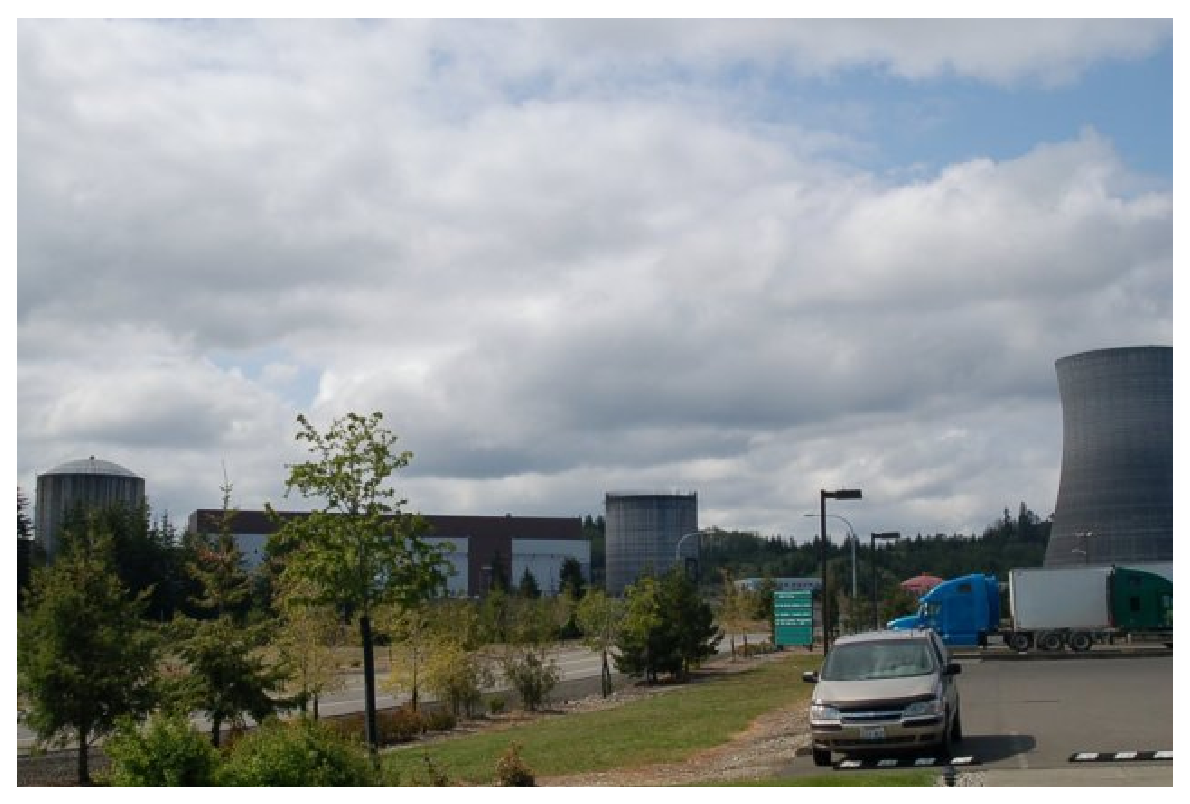
\includegraphics[width=3in]{i00001x01.eps} \hskip 20pt 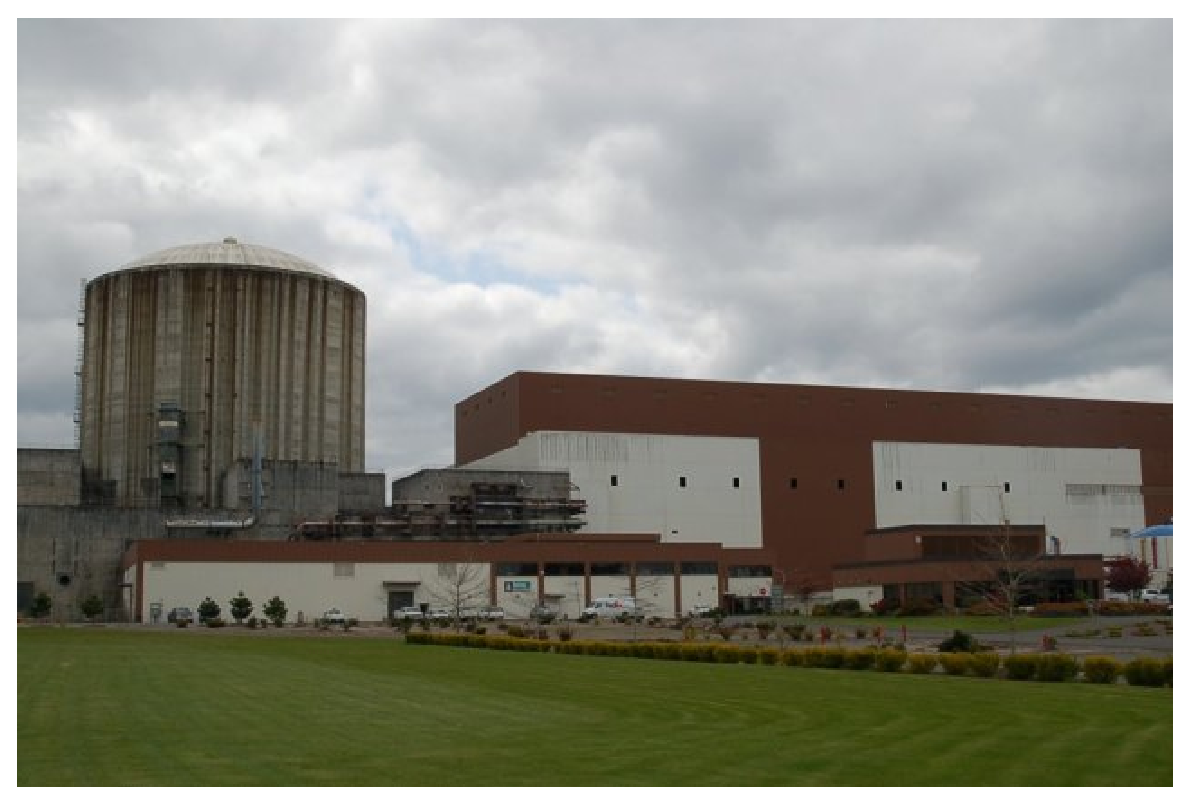
\includegraphics[width=3in]{i00001x06.eps}$$

\noindent
{\it Bilder tatt ved Satsop kjernekraftverk i Washington.}

$$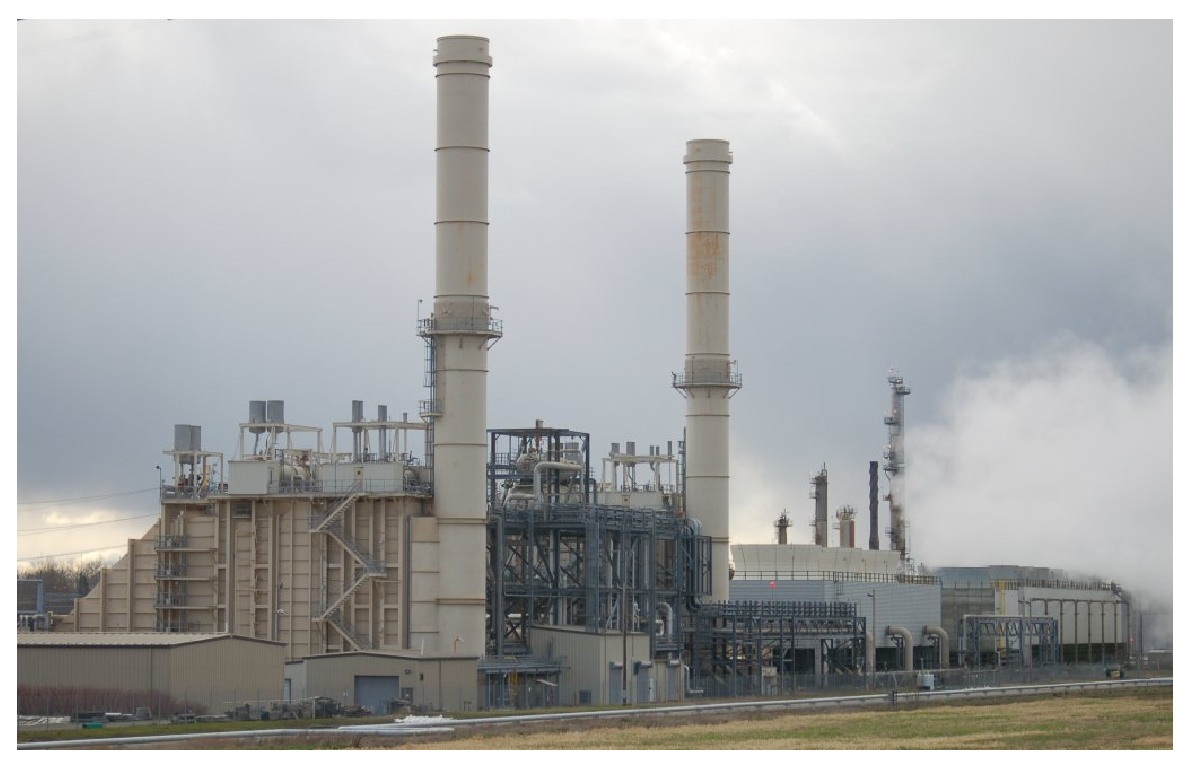
\includegraphics[width=4in]{i00001x29.eps}$$

\noindent
{\it Kombikraftverk (gassturbin + dampturbin) drevet av naturgass, i Ferndale, Washington.}

\filbreak

$$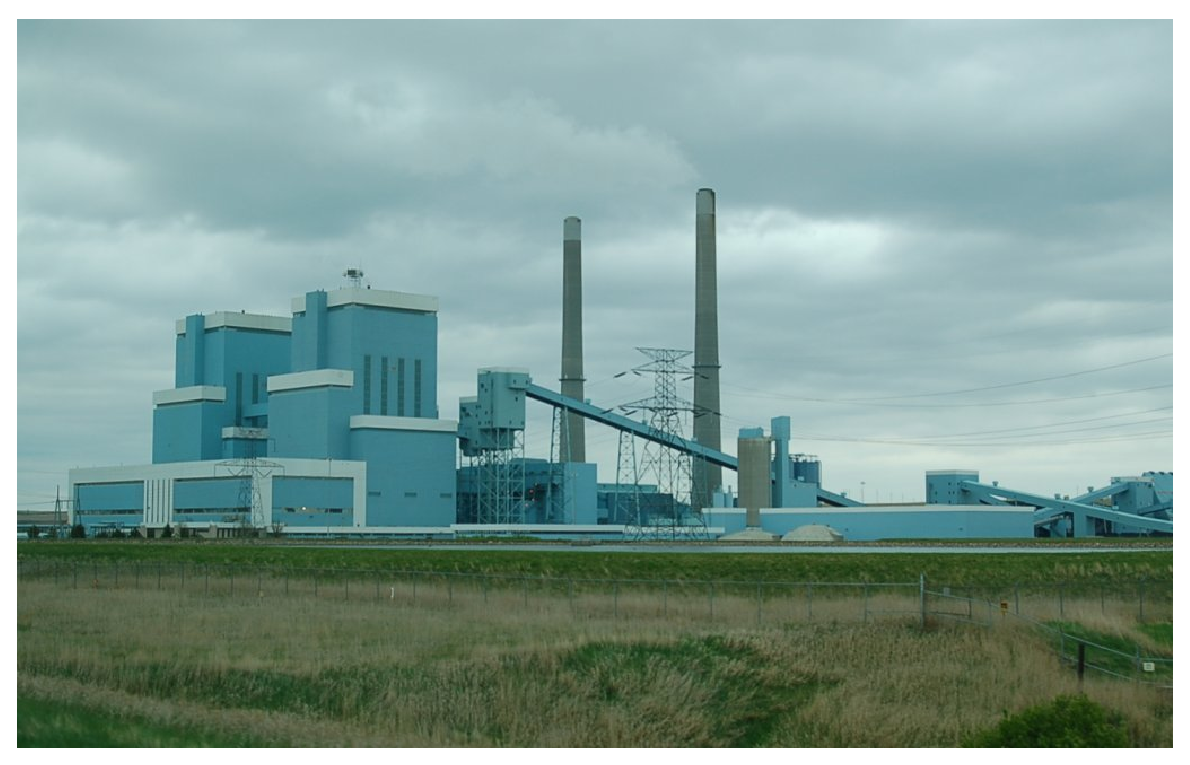
\includegraphics[width=5.5in]{i00001x33.eps}$$

\noindent
{\it Antelope Valley kullkraftverk i Beulah, North Dakota.}

$$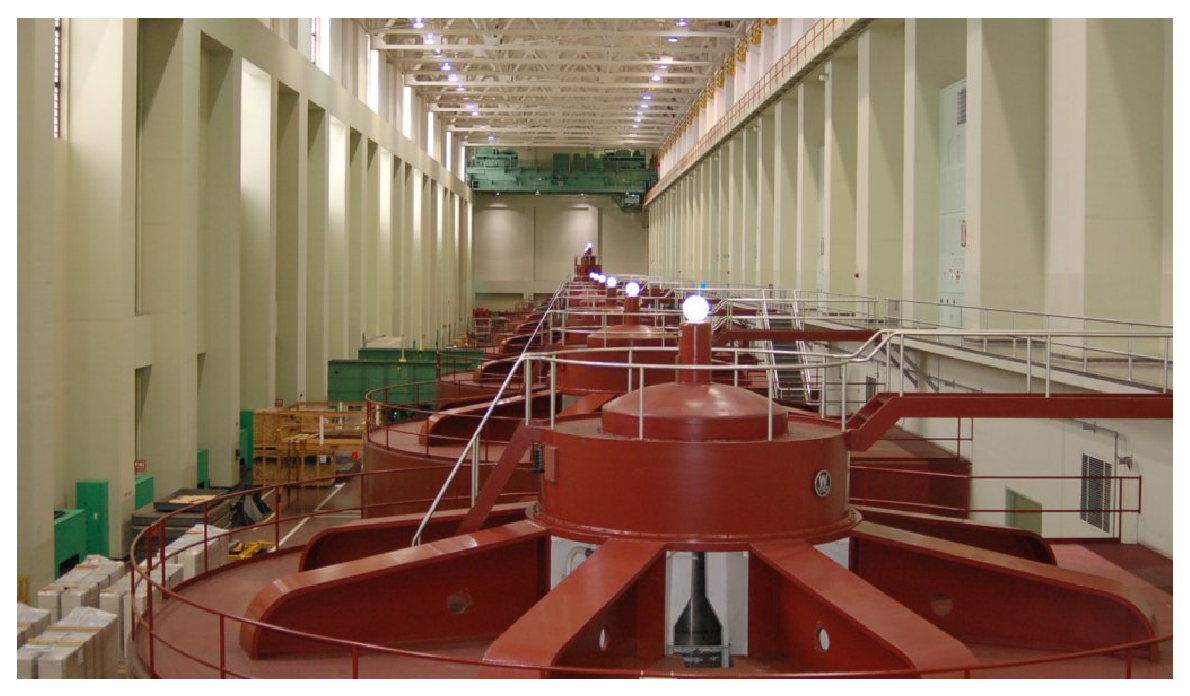
\includegraphics[width=5.5in]{i00001x37.eps}$$

\noindent
{\it Vannkraftturbiner ved Grand Coulee-dammen i Washington.}





\vskip 10pt \filbreak

\noindent
{\bf Olje- og naturgassleting/produksjon:}

$$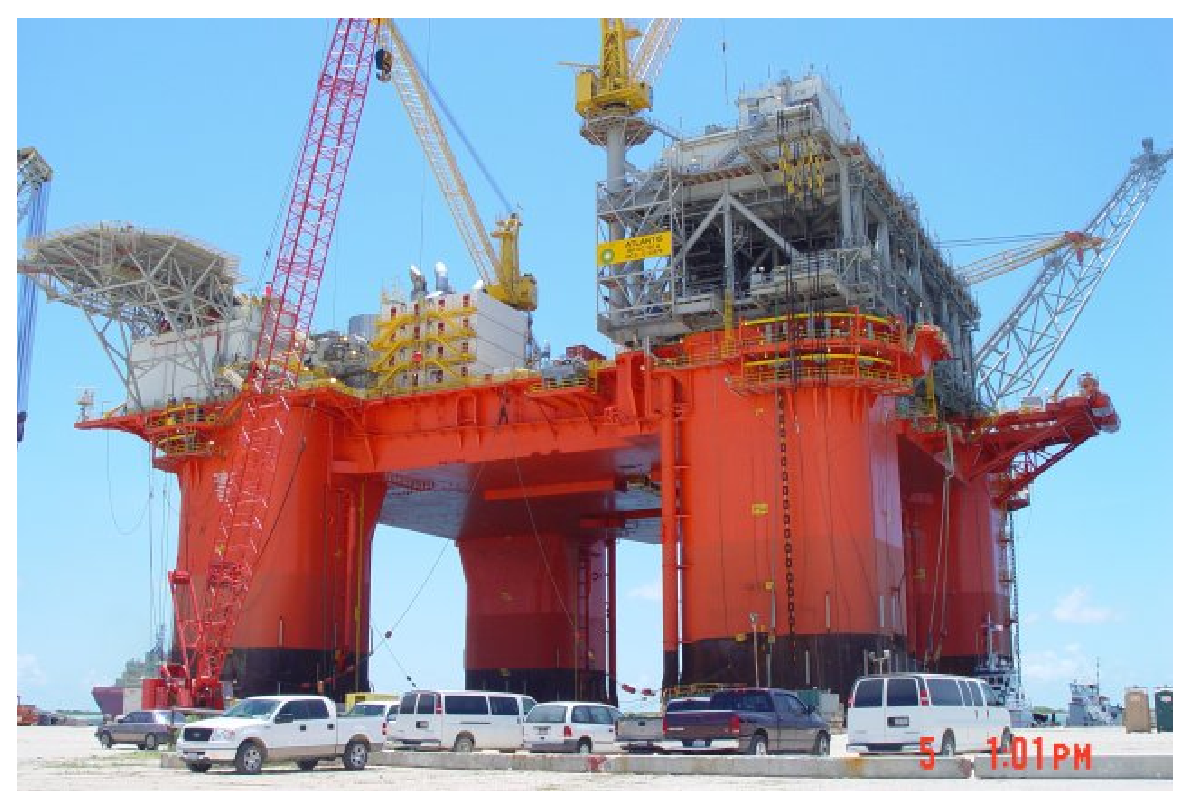
\includegraphics[width=5.25in]{i00001x19.eps}$$

\noindent
{\it BP Explorations ``Atlantis'' offshoreplattform under bygging.}

$$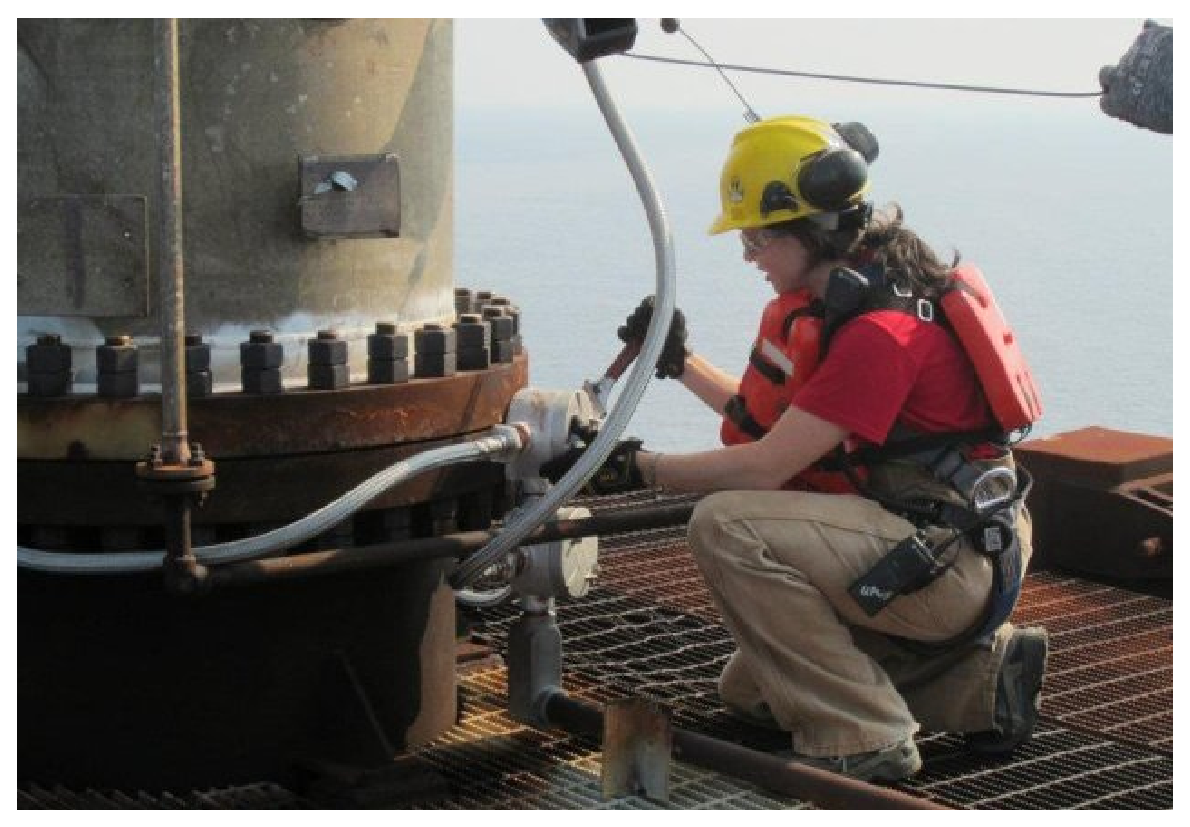
\includegraphics[width=5.25in]{i00001x28.eps}$$

\noindent
{\it BTC Instrumentation-graduate Paige reparerer flare-ignitors på en offshoreplattform i Mexicogolfen.}

\filbreak

$$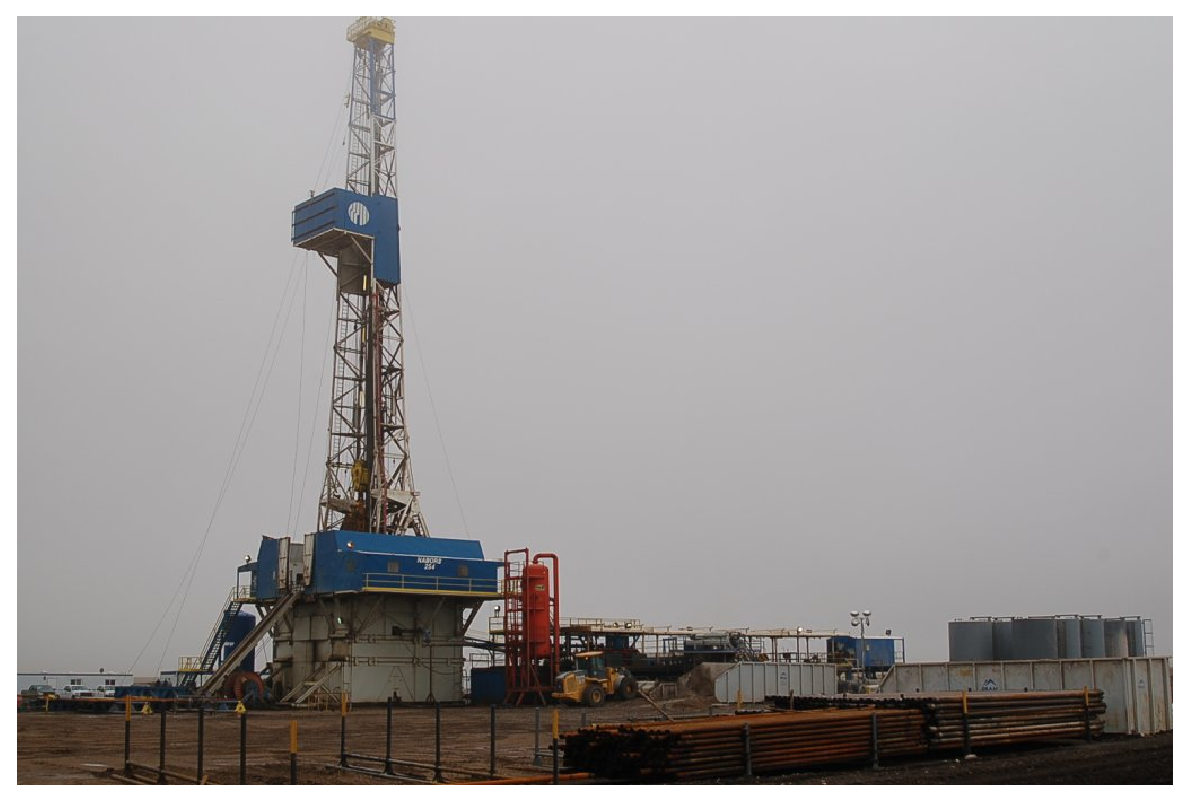
\includegraphics[width=3.5in]{i00001x36.eps}$$

\noindent
{\it Oljerigg i Bakken-oljefeltet (Stanley, North Dakota).  Disse riggene borer omtrent 2 miles ned, deretter horisontalt og frakturerer skiferlaget for å la olje sive ut og bli samlet inn.}

$$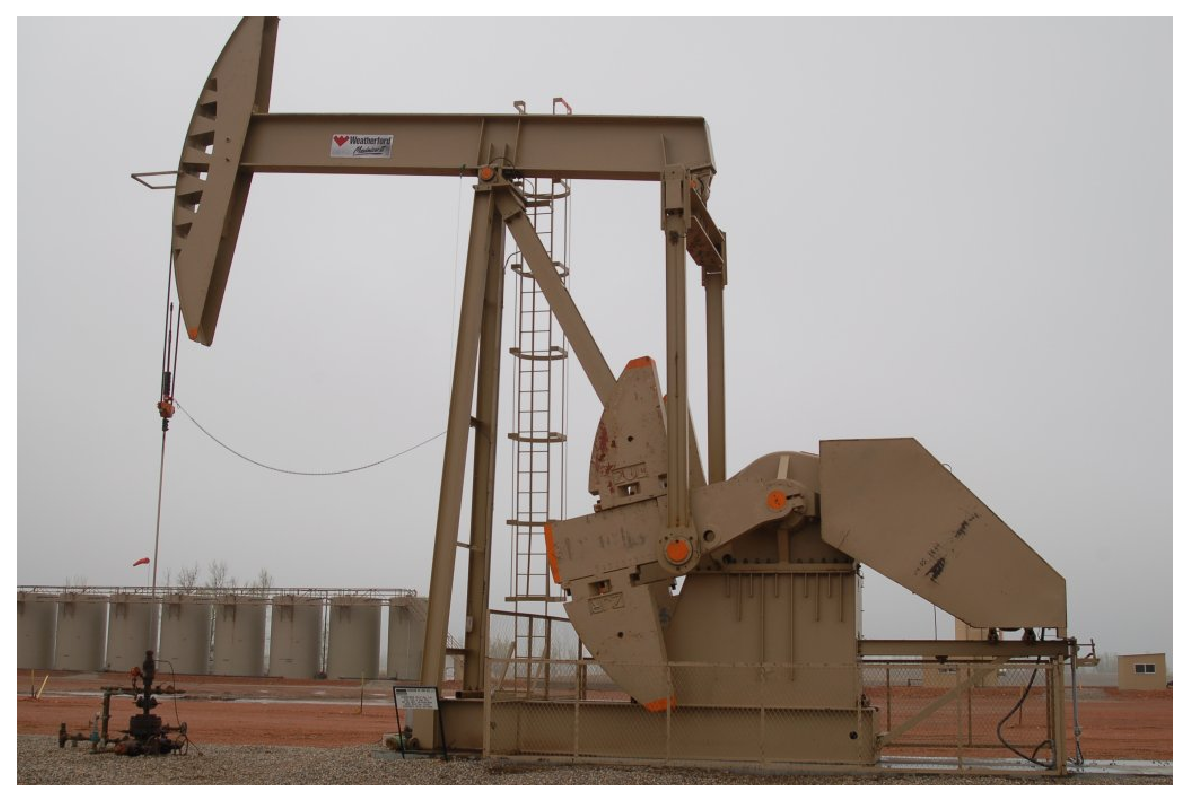
\includegraphics[width=3.5in]{i00001x34.eps}$$

\noindent
{\it Oljehode og pumpe i Stanley, North Dakota.}







\vskip 10pt \filbreak

\noindent
{\bf Oljeraffinering:}

$$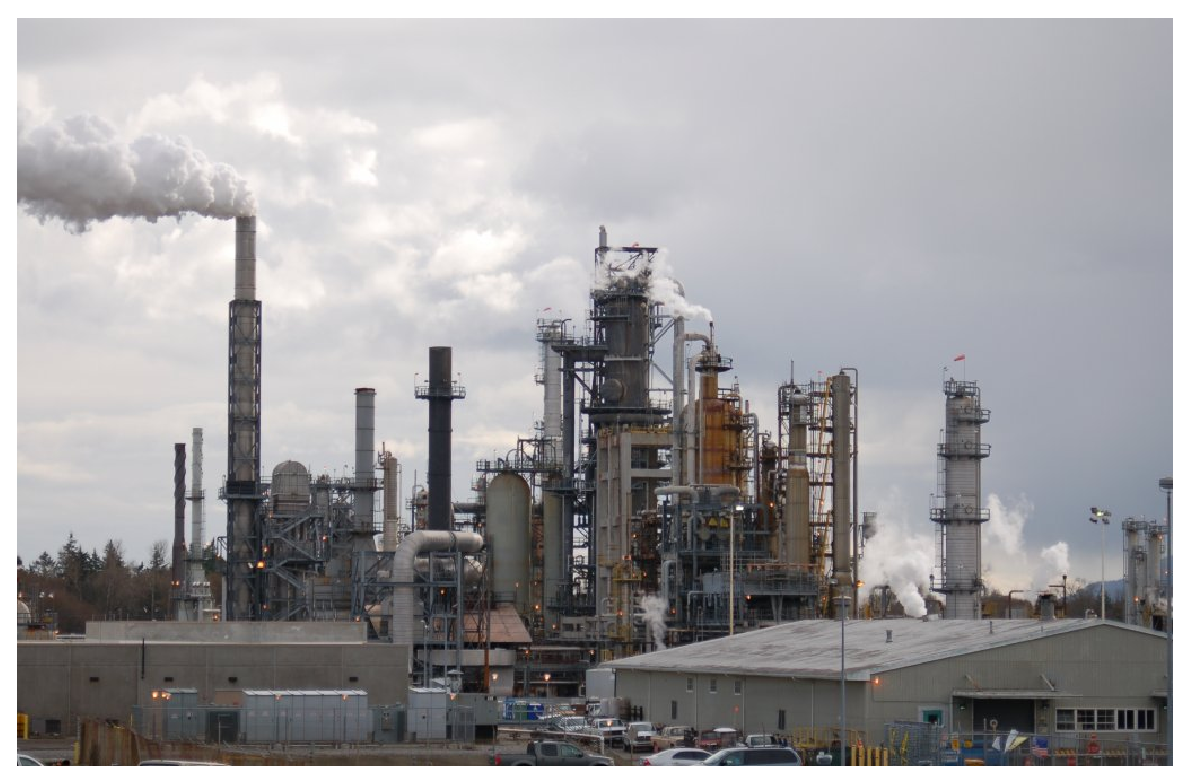
\includegraphics[width=3.5in]{i00001x30.eps}$$

\noindent
{\it Phillips66-raffineriet i Ferndale, Washington.}






\vskip 10pt \filbreak

\noindent
{\bf Kullgassifisering:}

$$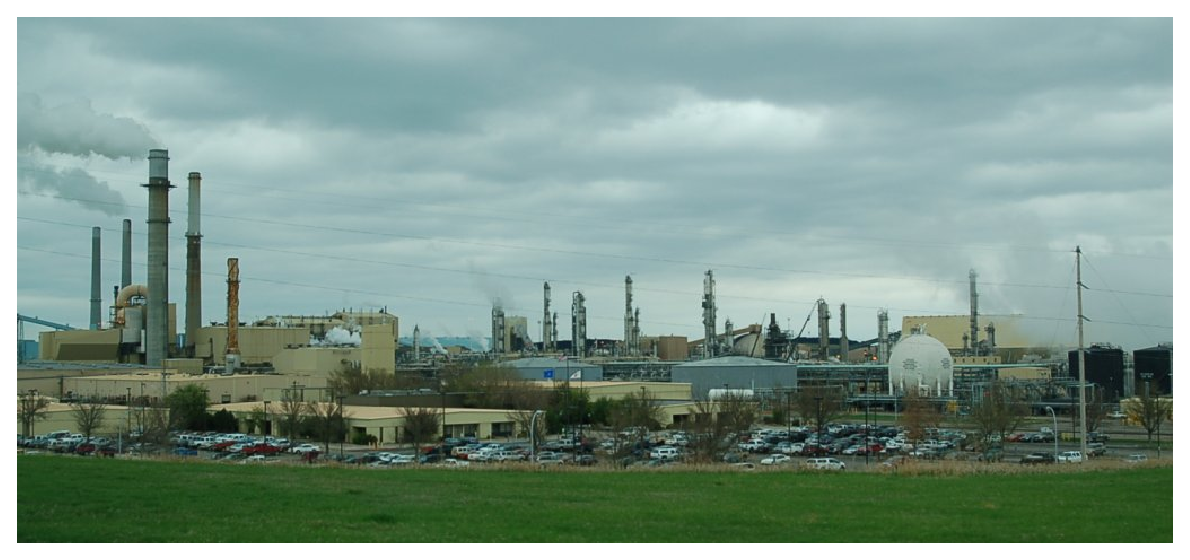
\includegraphics[width=5.5in]{i00001x35.eps}$$

\noindent
{\it Dakota Gasification-anlegget i Beulah, North Dakota.  Produserer syntetisk naturgass, ammoniakk og en rekke andre høyverdige kjemiske produkter fra kull.  En majoritet av karbondioksidet som produseres i denne prosessen blir fanget og ført i rør til oljefelt i Canada for økt utvinning, hvor CO$_{2}$-gassen ender opp lagret i underjordiske brønner.}






\vskip 10pt \filbreak

\noindent
{\bf Kjemisk prosessindustri:}

$$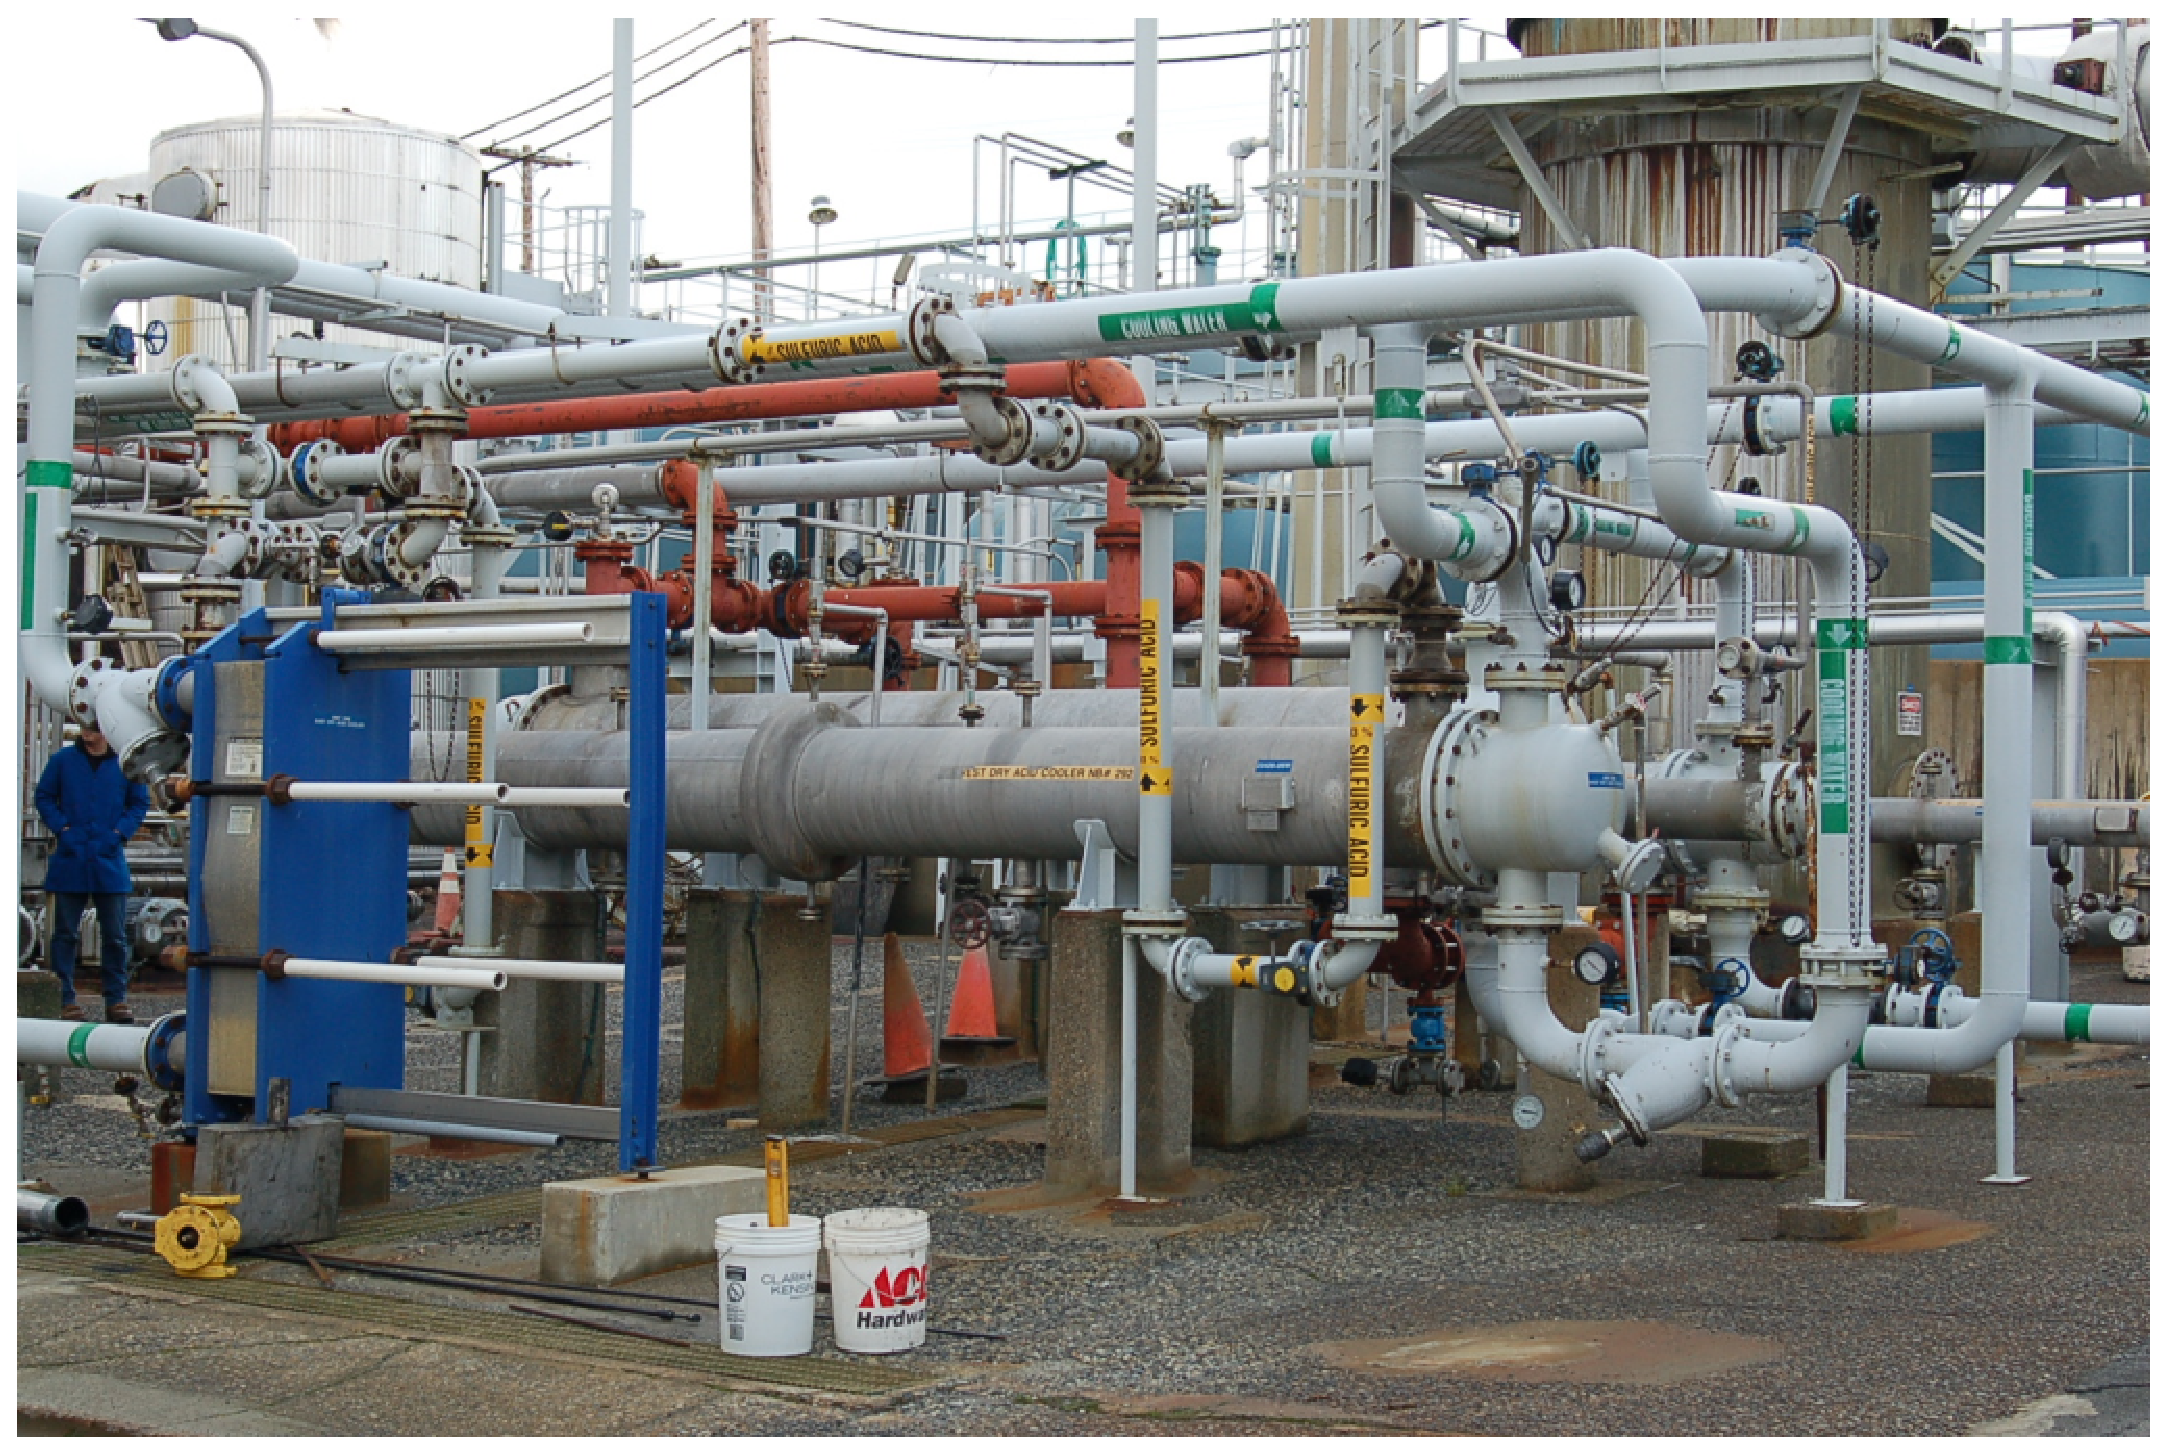
\includegraphics[width=3.5in]{i00001x39.eps}$$

\noindent
{\it Chemtrade Solutions' anlegg for reprosessering av svovelsyre i Anacortes, Washington.  Dette anlegget mottar ``brukt'' svovelsyre fra to oljeraffinerier (alkyleringsenheter, hvor svovelsyre brukes som flytende katalysator) og reprosesserer den forurensede syren til nesten ren syre for videresalg og gjenbruk i raffineriene.}






\vskip 10pt \filbreak

\noindent
{\bf Tremasse- og papirproduksjon:}

$$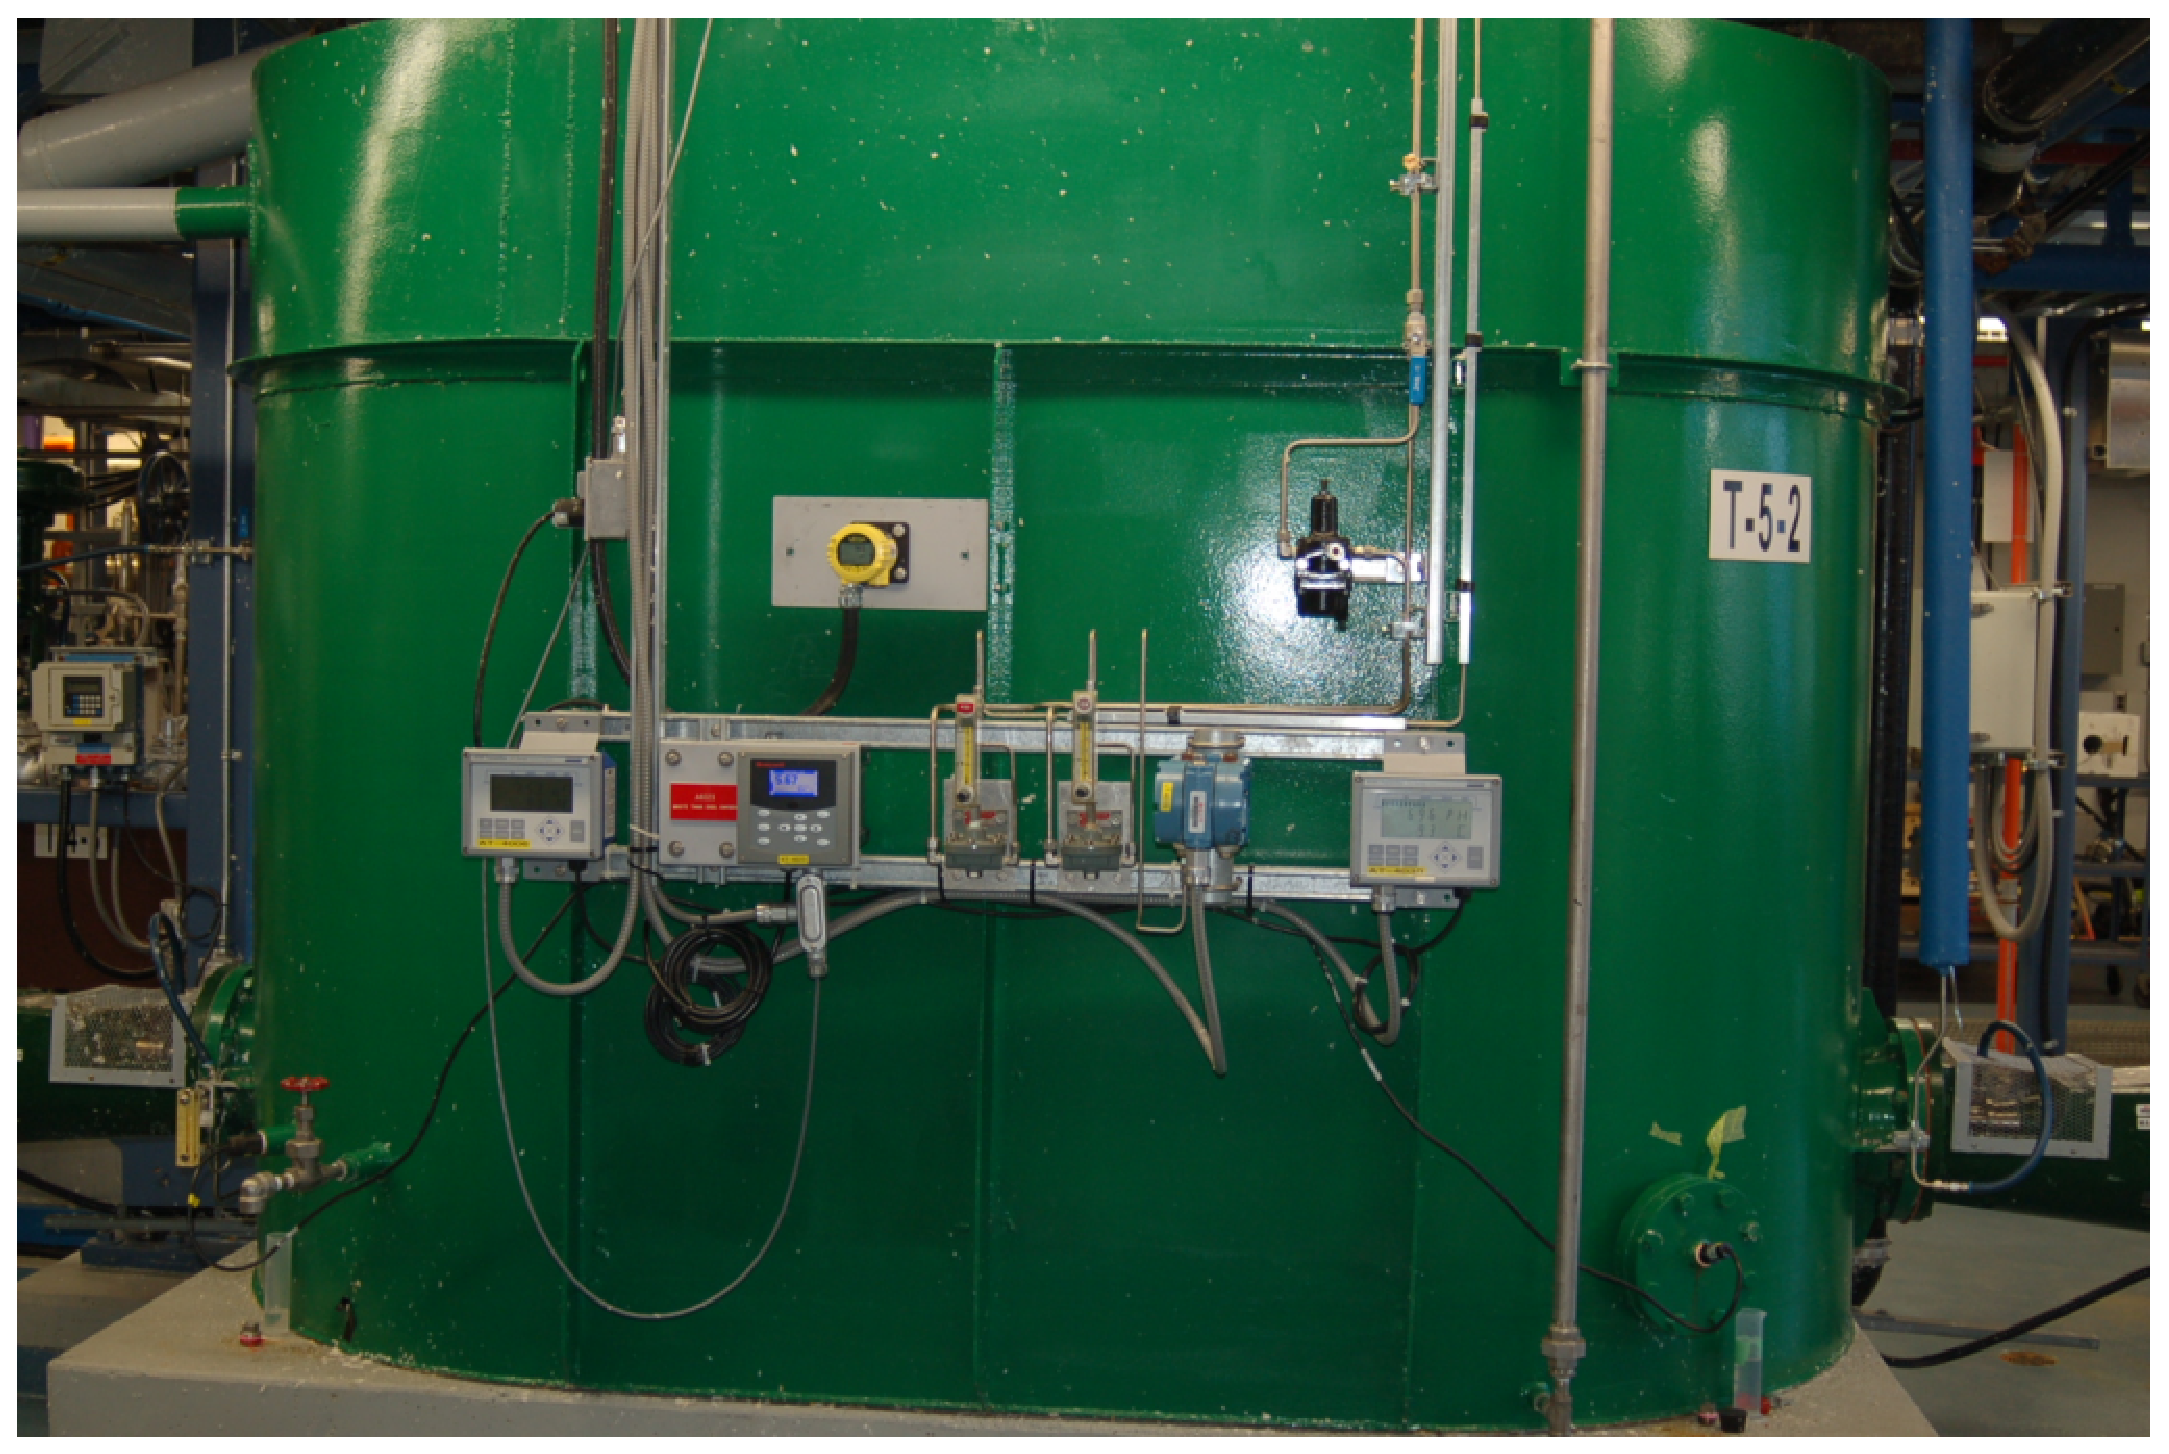
\includegraphics[width=3.5in]{i00001x40.eps}$$

\noindent
{\it Dette er ``blend chest'' i en liten pulp-operasjon, der ulike kvaliteter av tremasse blandes sammen for å oppnå riktig blanding for papirproduksjon.}








\vskip 10pt \filbreak

\noindent
{\bf Farmasøytisk produksjon:}

$$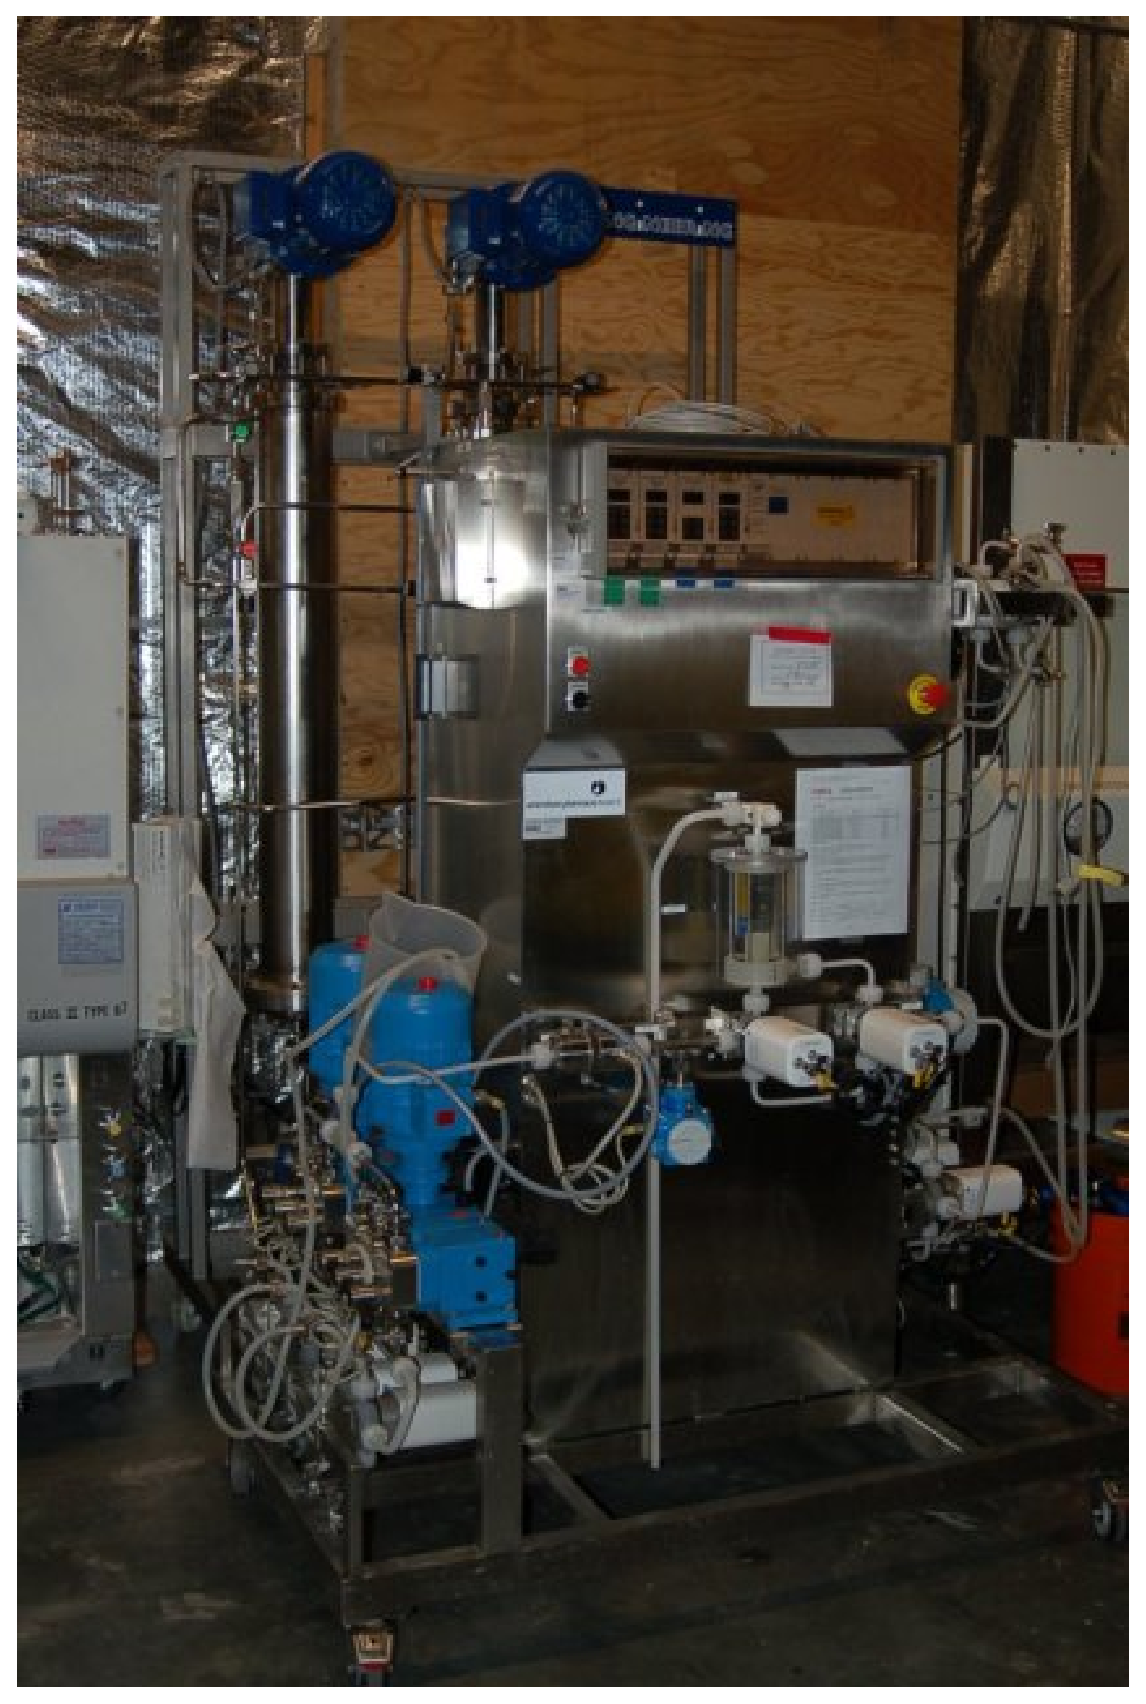
\includegraphics[width=3in]{i00001x02.eps} \hskip 20pt 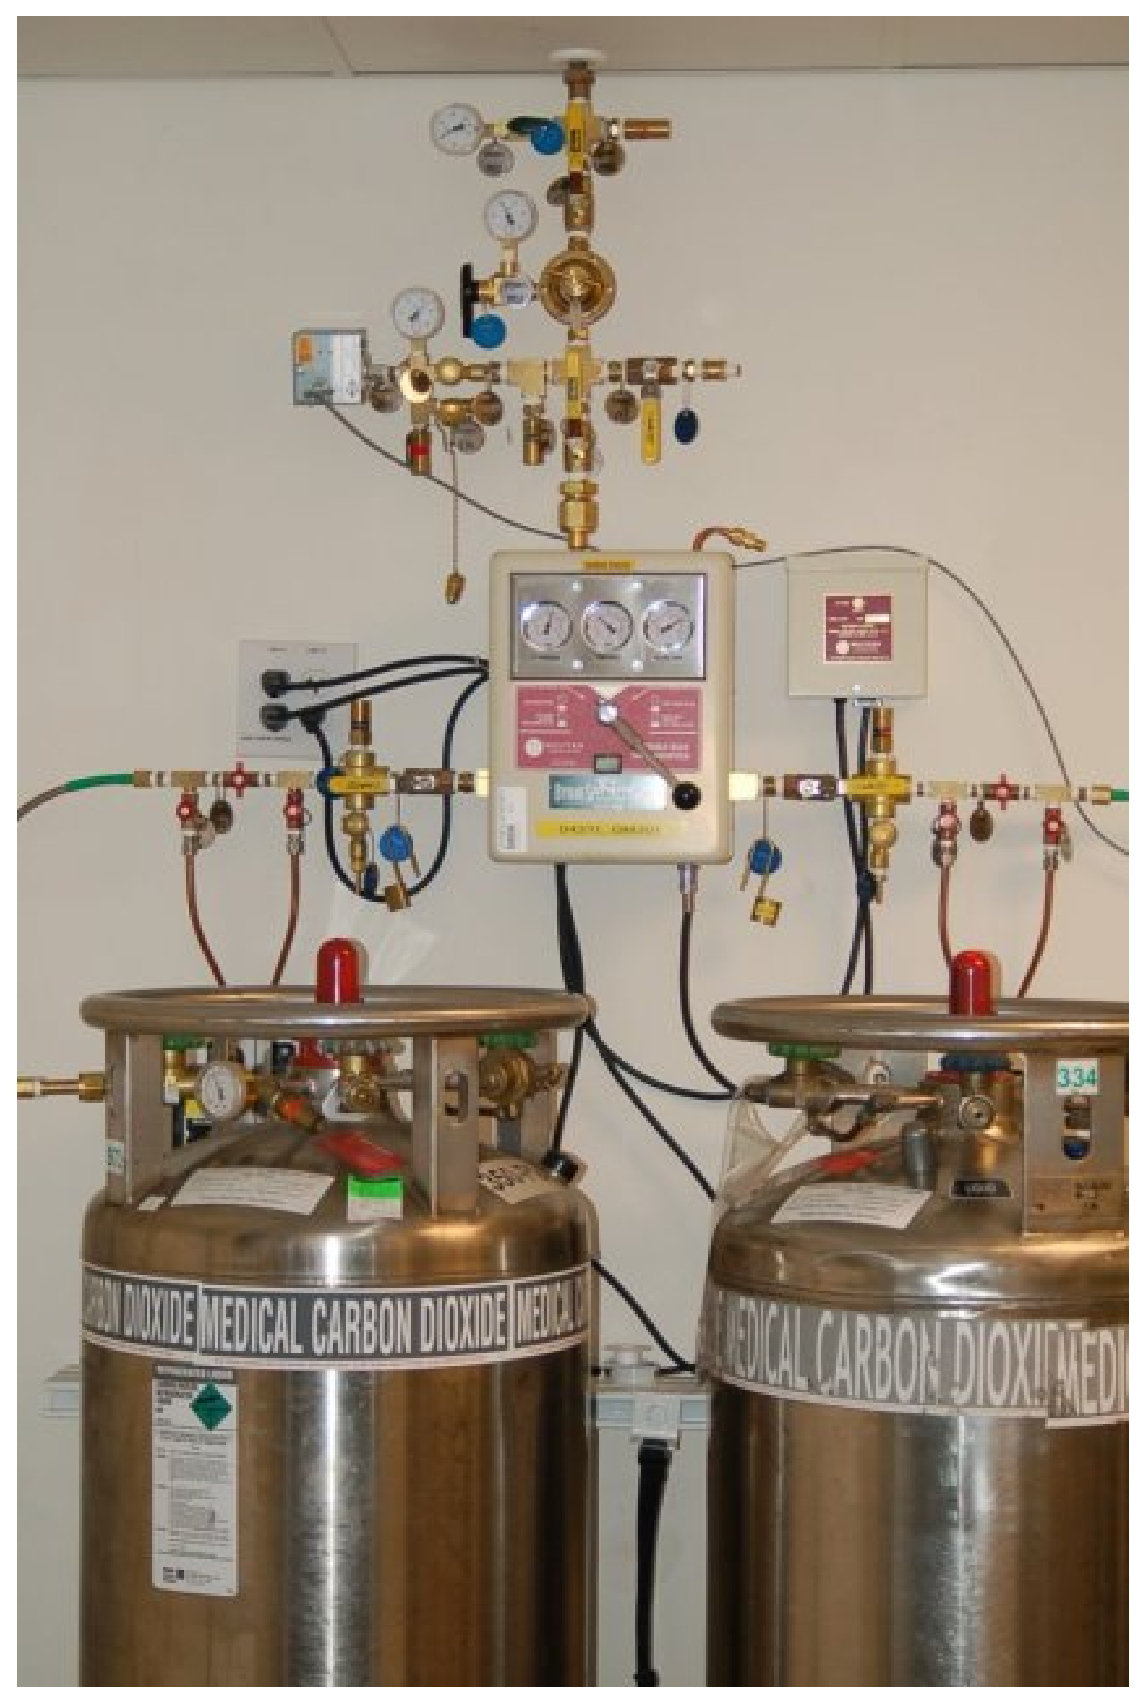
\includegraphics[width=3in]{i00001x05.eps}$$

\noindent
{\it Bilder tatt hos Zymogenetics i Seattle.  Beklager -- de lot meg ikke ta noen bilder av de virkelig kule tingene!}






\vskip 10pt \filbreak

\noindent
{\bf Naturgasskomprimering og -distribusjon:}

$$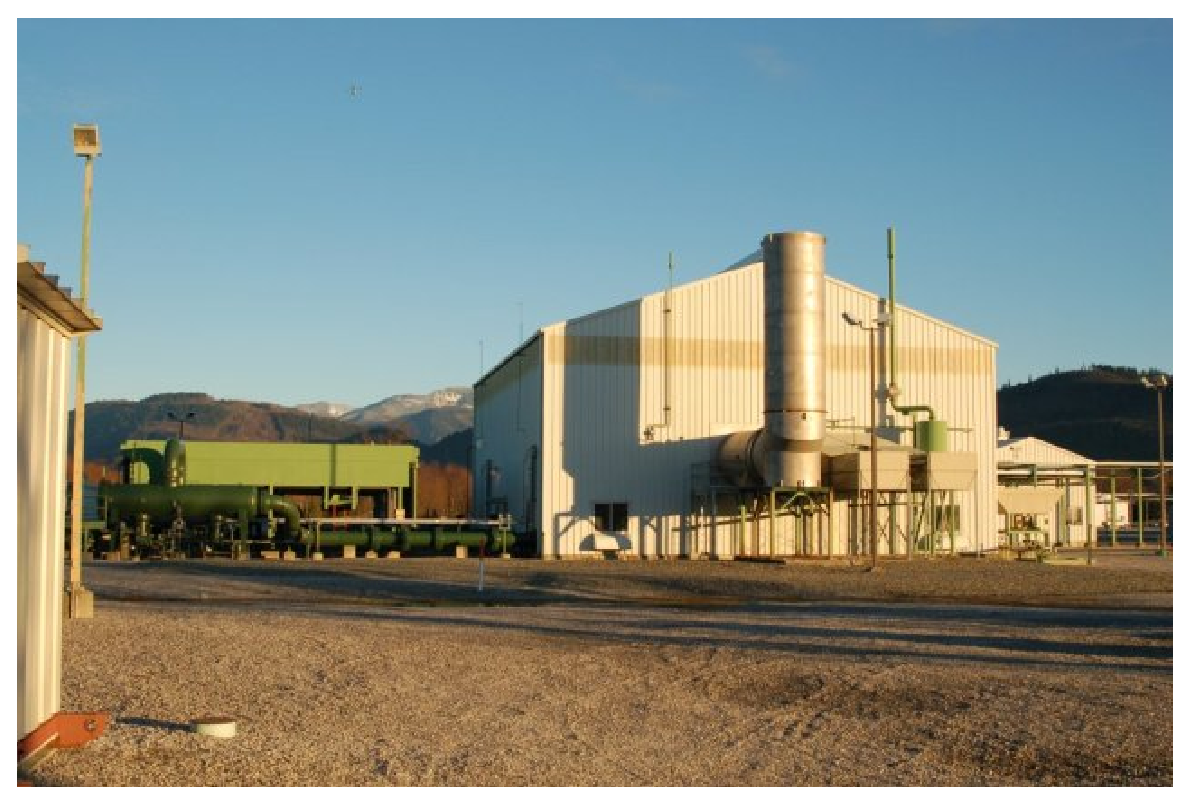
\includegraphics[width=3.5in]{i00001x03.eps}$$

\noindent
{\it Williams Northwest Pipeline sitt gasskompresjonsanlegg i Sumas, Washington.}

$$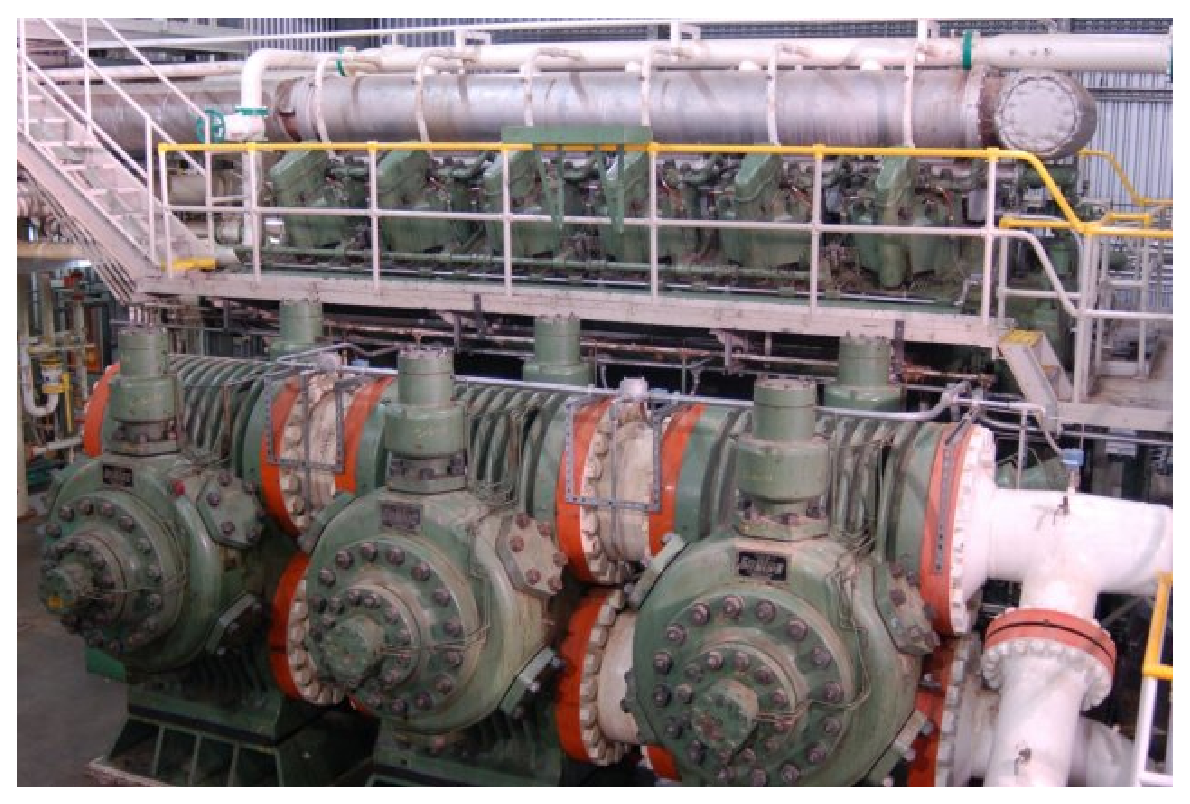
\includegraphics[width=3.5in]{i00001x04.eps}$$

\noindent
{\it Stor stempelmotor brukt til å komprimere naturgass.}






\vskip 10pt \filbreak

\noindent
{\bf Næringsmiddelindustri og emballering:}

$$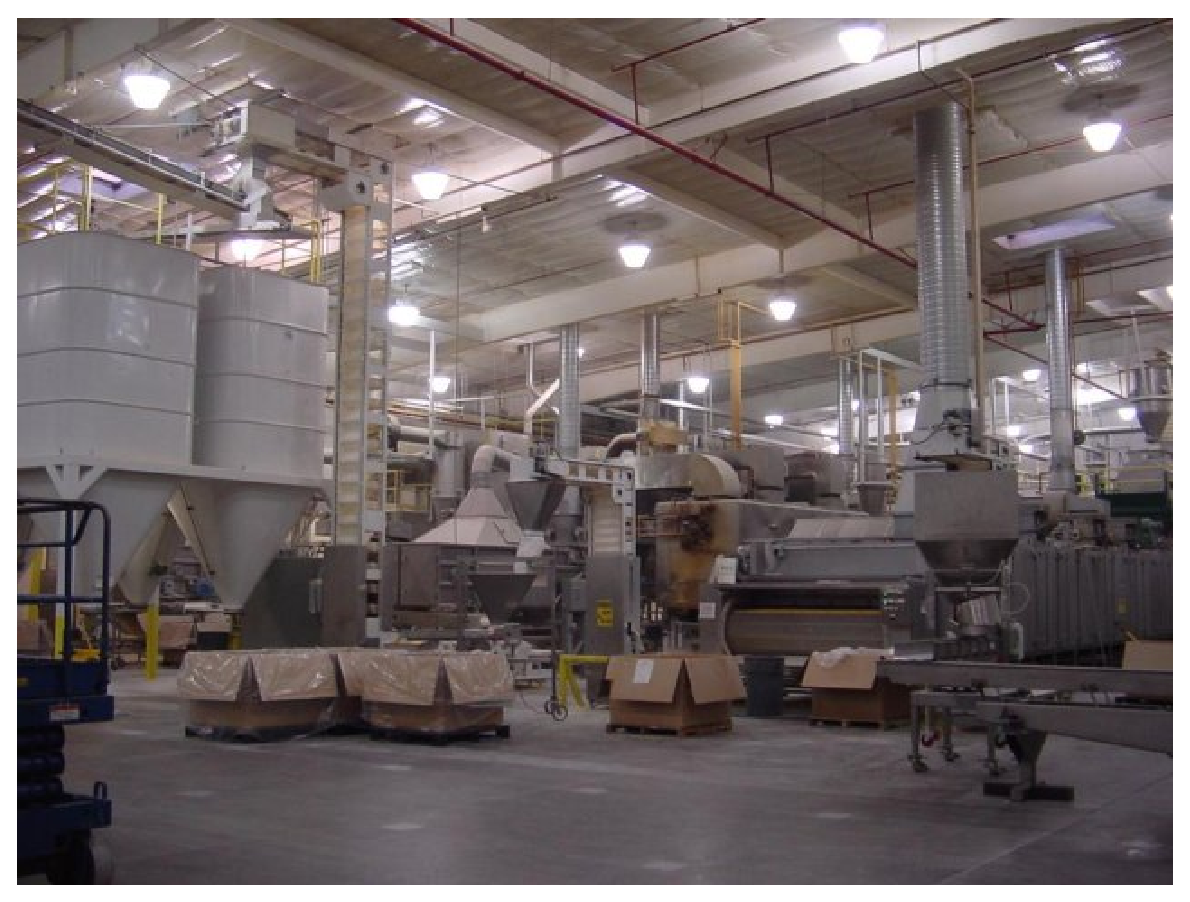
\includegraphics[width=3.5in]{i00001x07.eps}$$

\noindent
{\it Produksjonsgulv hos Nature's Path Foods i Blaine, Washington.}

$$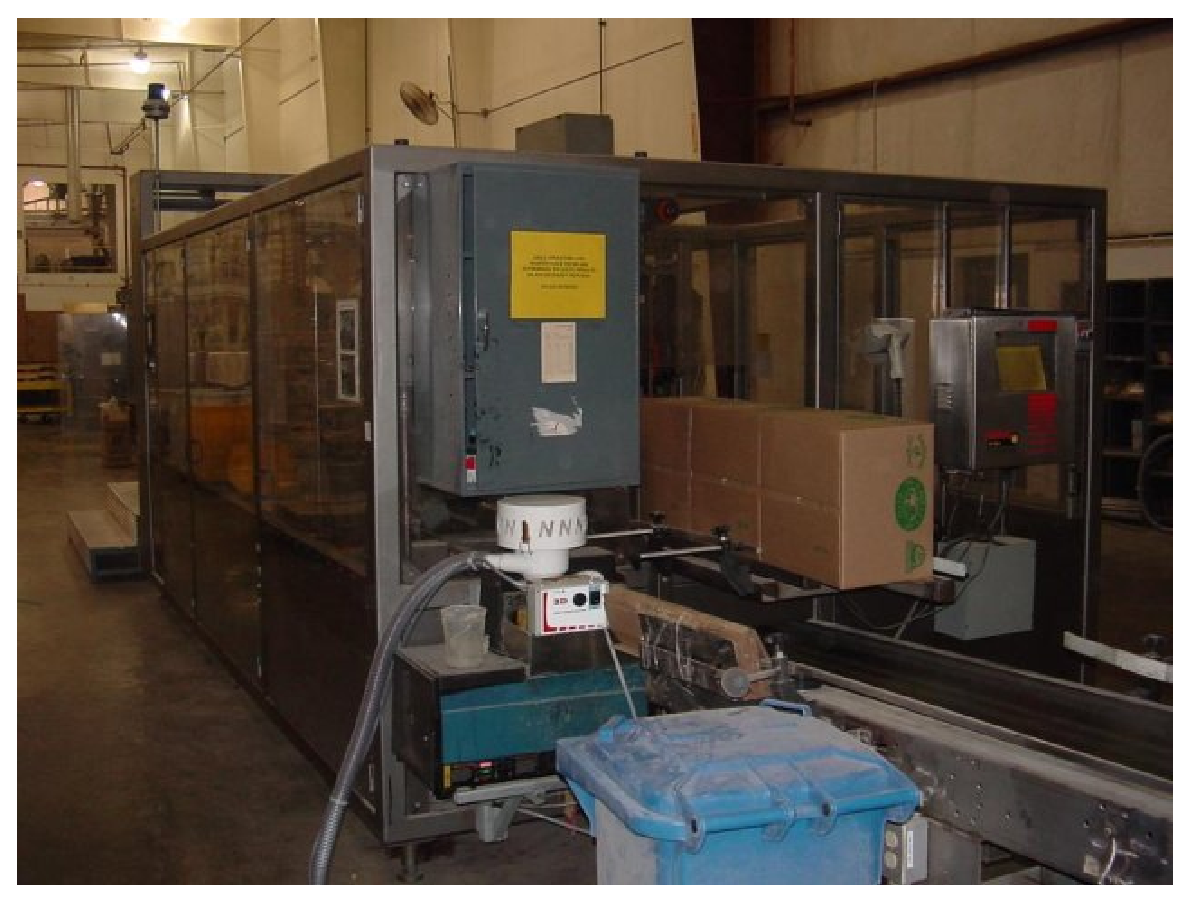
\includegraphics[width=3.5in]{i00001x08.eps}$$

\noindent
{\it Automatisert pakkemaskin for frokostblanding.}






\vskip 10pt \filbreak

\noindent
{\bf Alkoholproduksjon og tapping:}

$$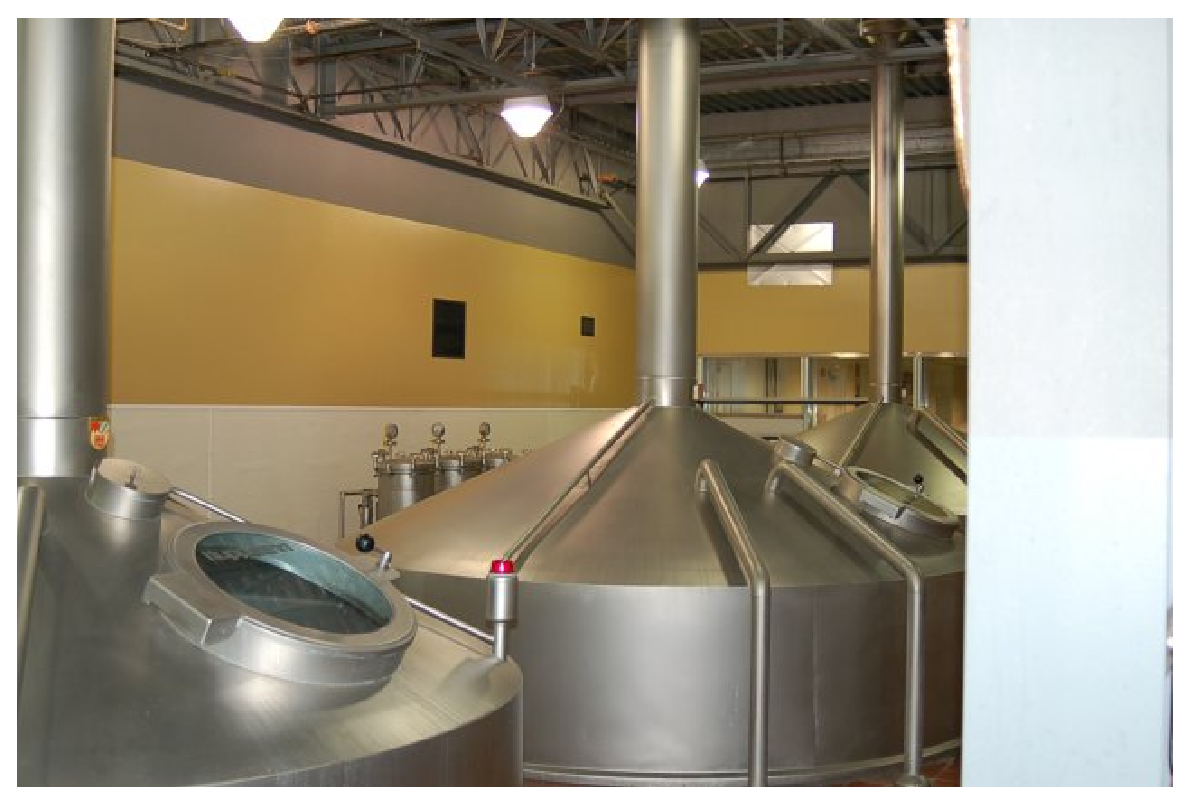
\includegraphics[width=3.5in]{i00001x27.eps}$$
$$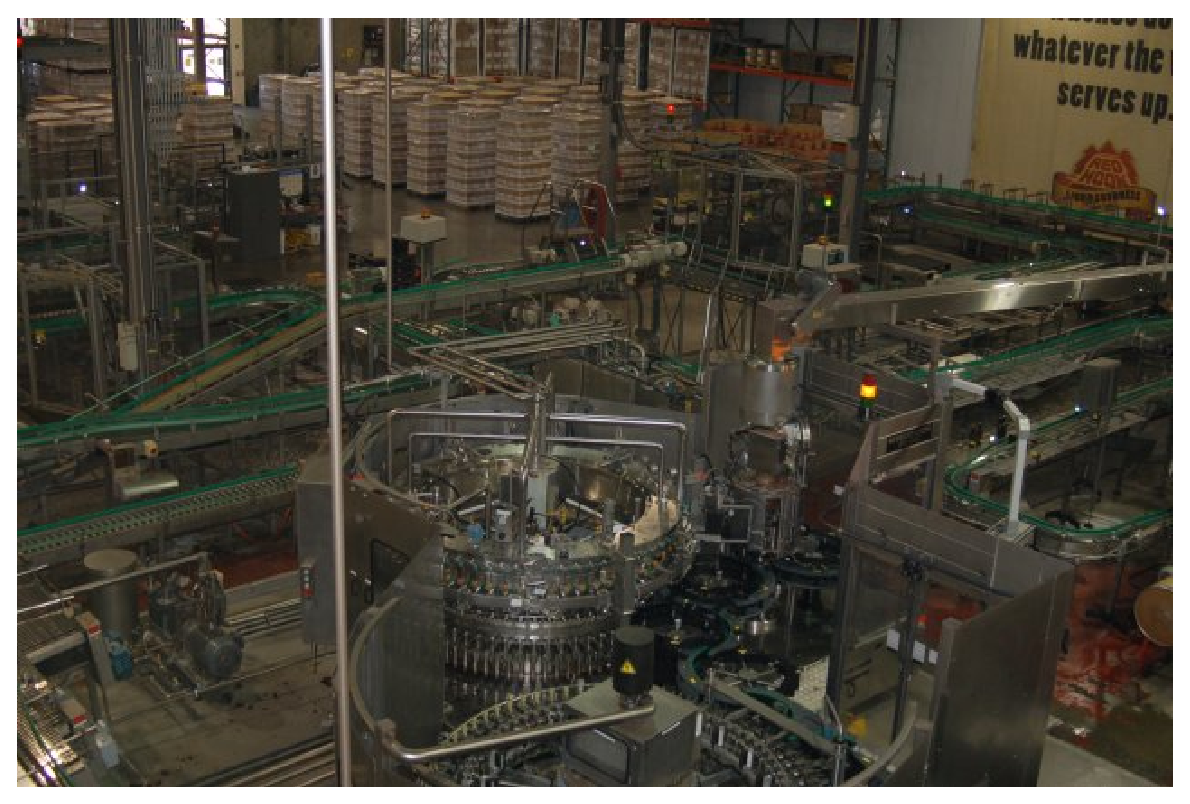
\includegraphics[width=3.5in]{i00001x26.eps}$$

\noindent
{\it Mesketanker og tappe-linje hos RedHook Brewery i Woodinville, Washington.}






\vskip 10pt \filbreak

\noindent
{\bf Kommunal vann- og avløpsrensing:}

$$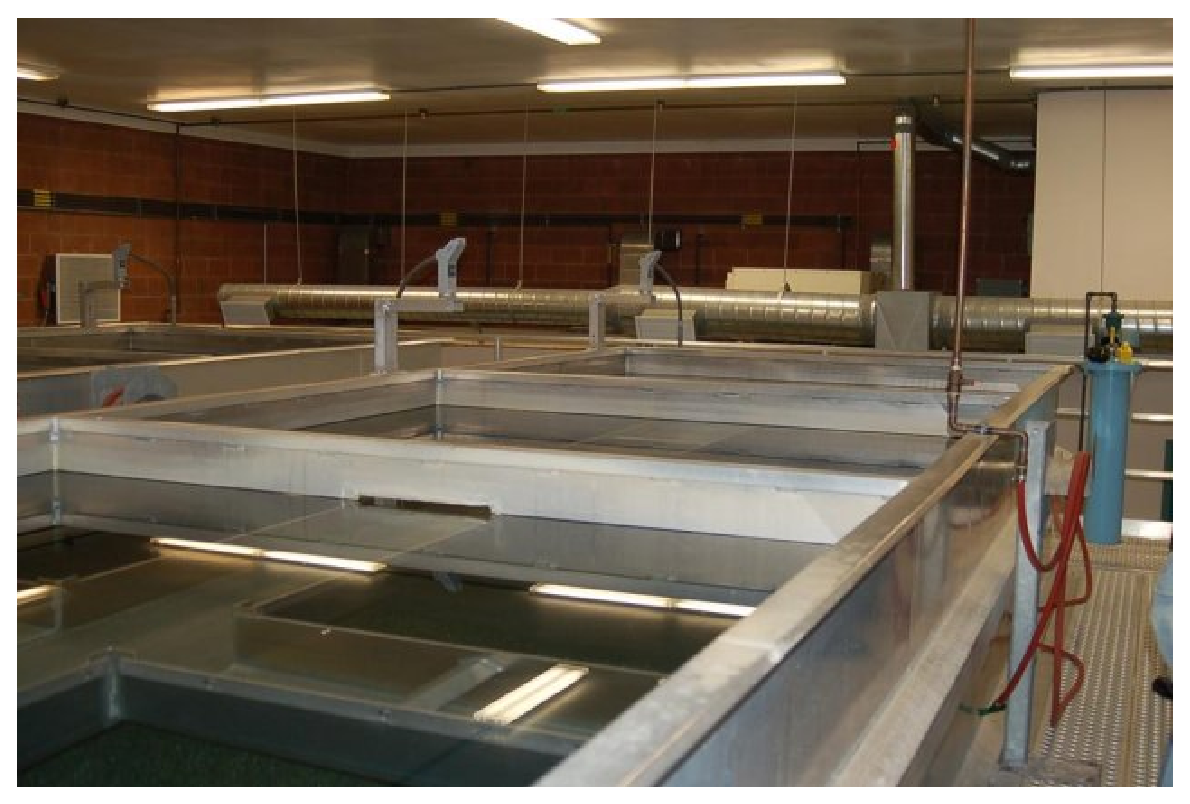
\includegraphics[width=3.5in]{i00001x09.eps}$$

\noindent
{\it Filtrering av drikkevann i byen Arlington, Washington.}

$$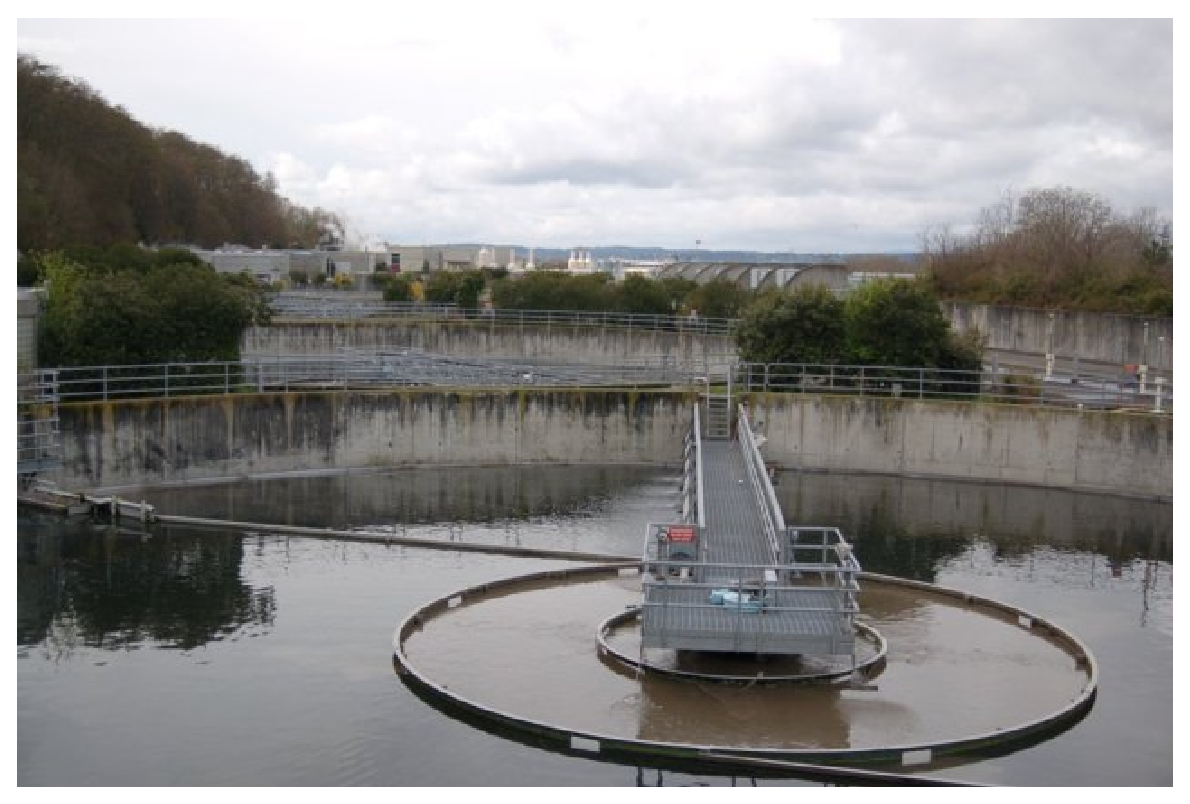
\includegraphics[width=3.5in]{i00001x10.eps}$$

\noindent
{\it Klarifisering av avløpsvann ved West Point-anlegget i King County (Seattle), Washington.}






\vskip 10pt \filbreak

\noindent
{\bf Elektrisk kraftdistribusjon:}

$$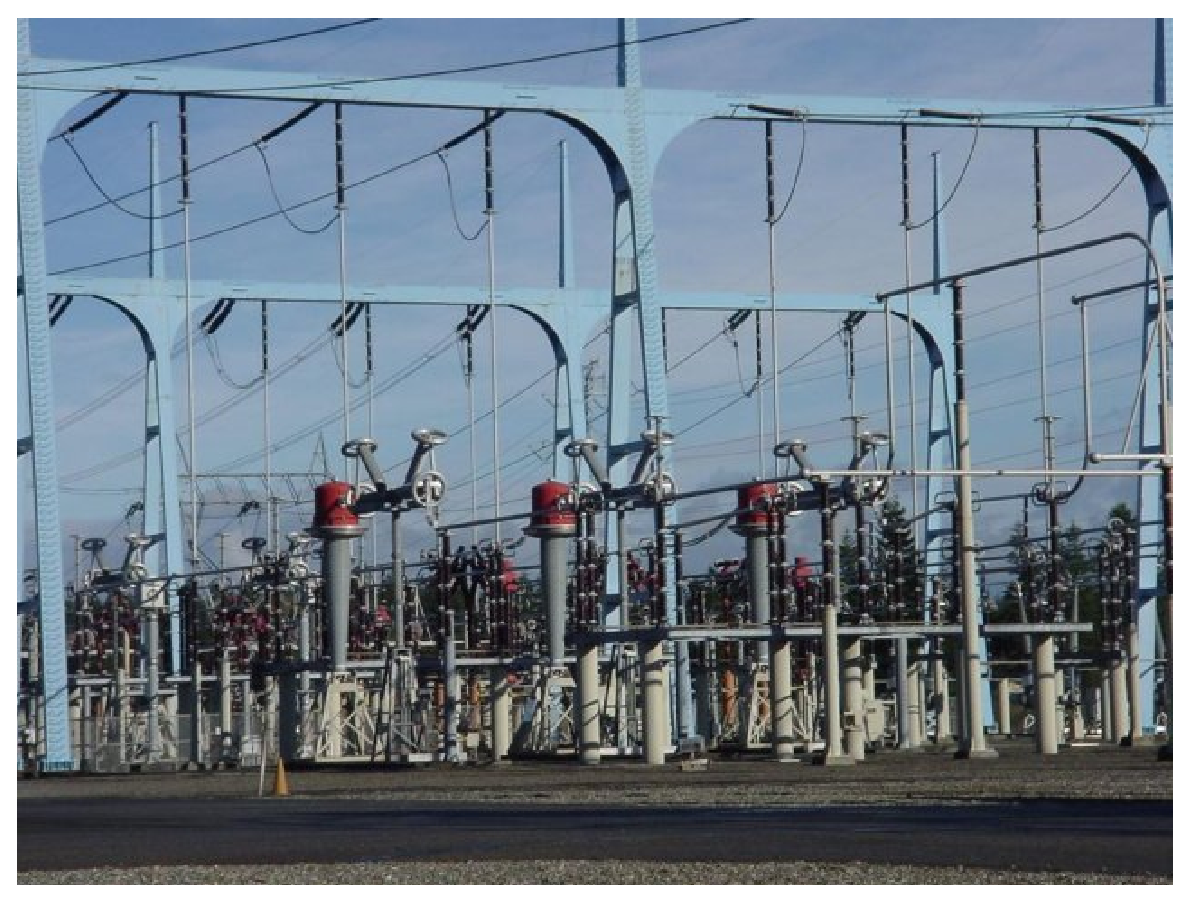
\includegraphics[width=3.5in]{i00001x11.eps}$$
$$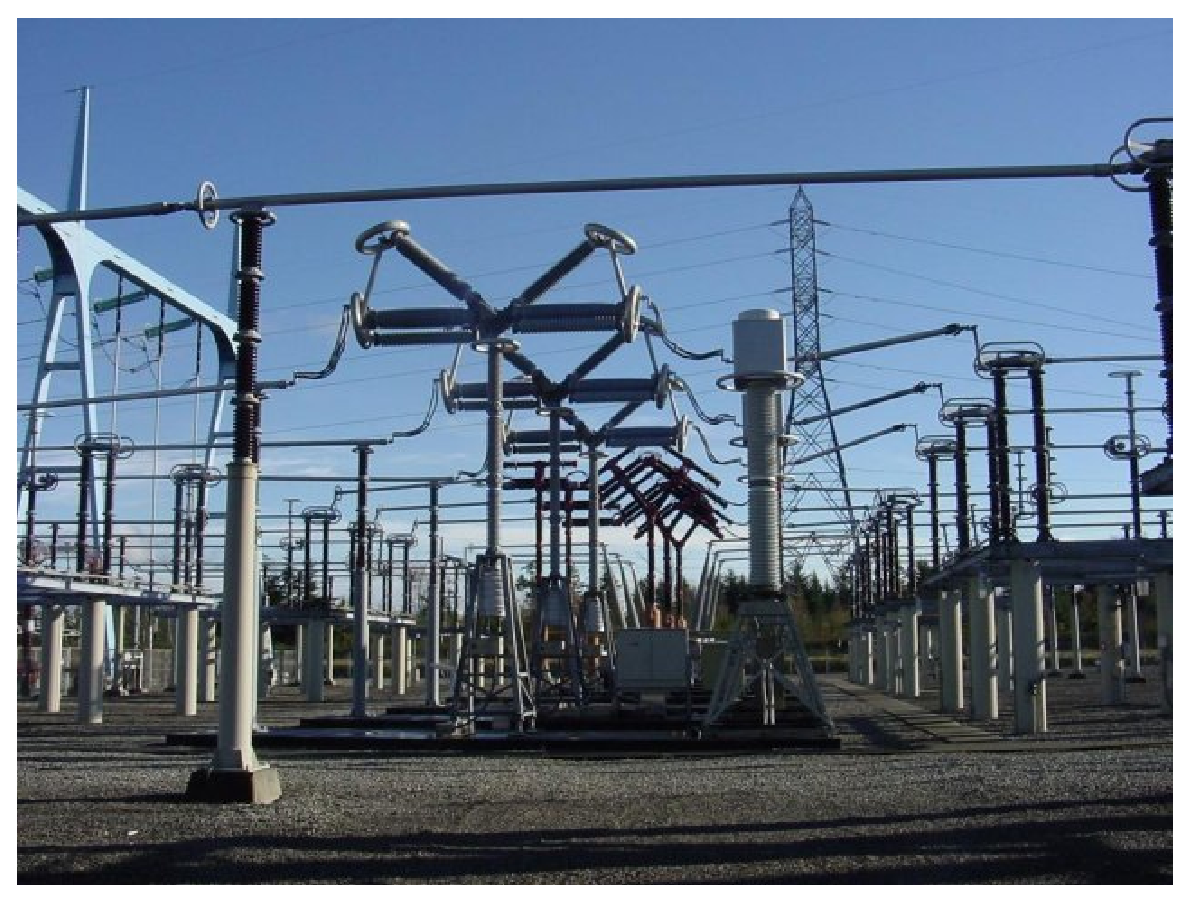
\includegraphics[width=3.5in]{i00001x12.eps}$$

\noindent
{\it Bonneville Power Administration sin Custer, Washington transformatorstasjon (500 000 volt).}






\vskip 10pt \filbreak

\noindent
{\bf Sagbruk og trebehandling:}

$$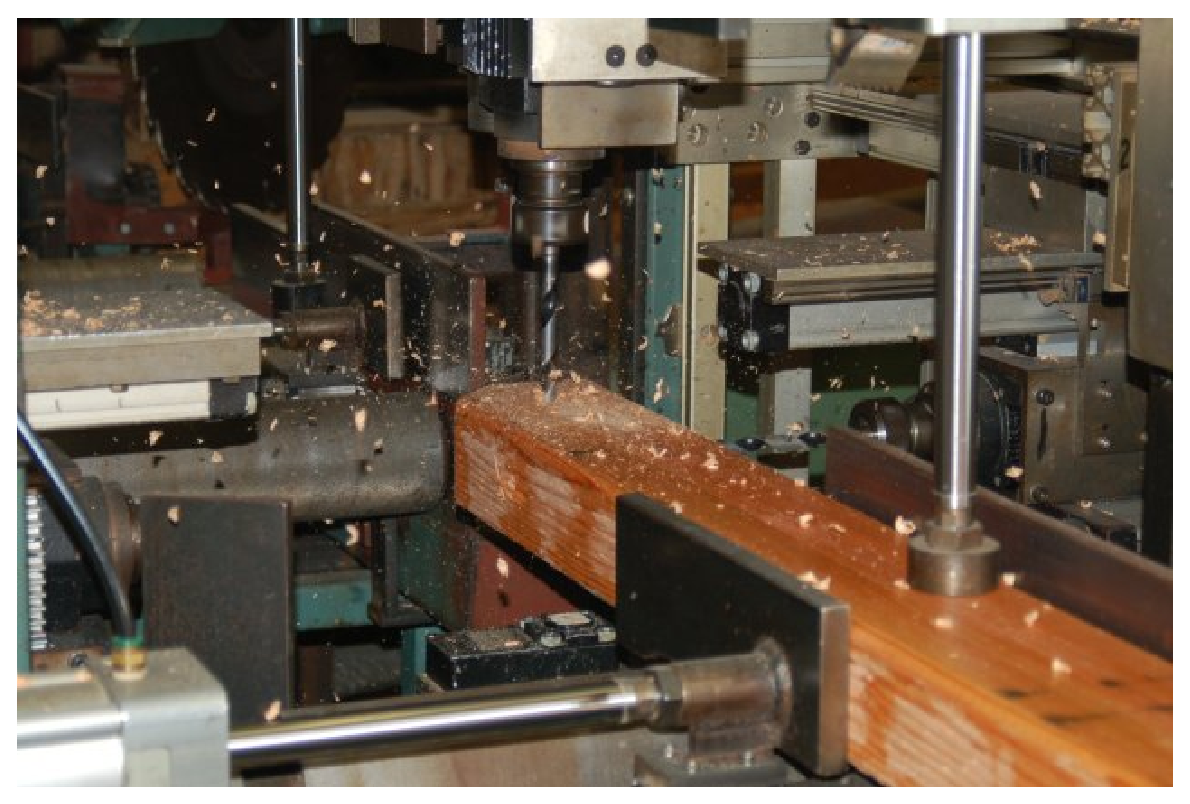
\includegraphics[width=3.5in]{i00001x16.eps}$$

\noindent
{\it En datastyrt boremaskin lager hull i en tverrbjelke til kraftlinjer.}

$$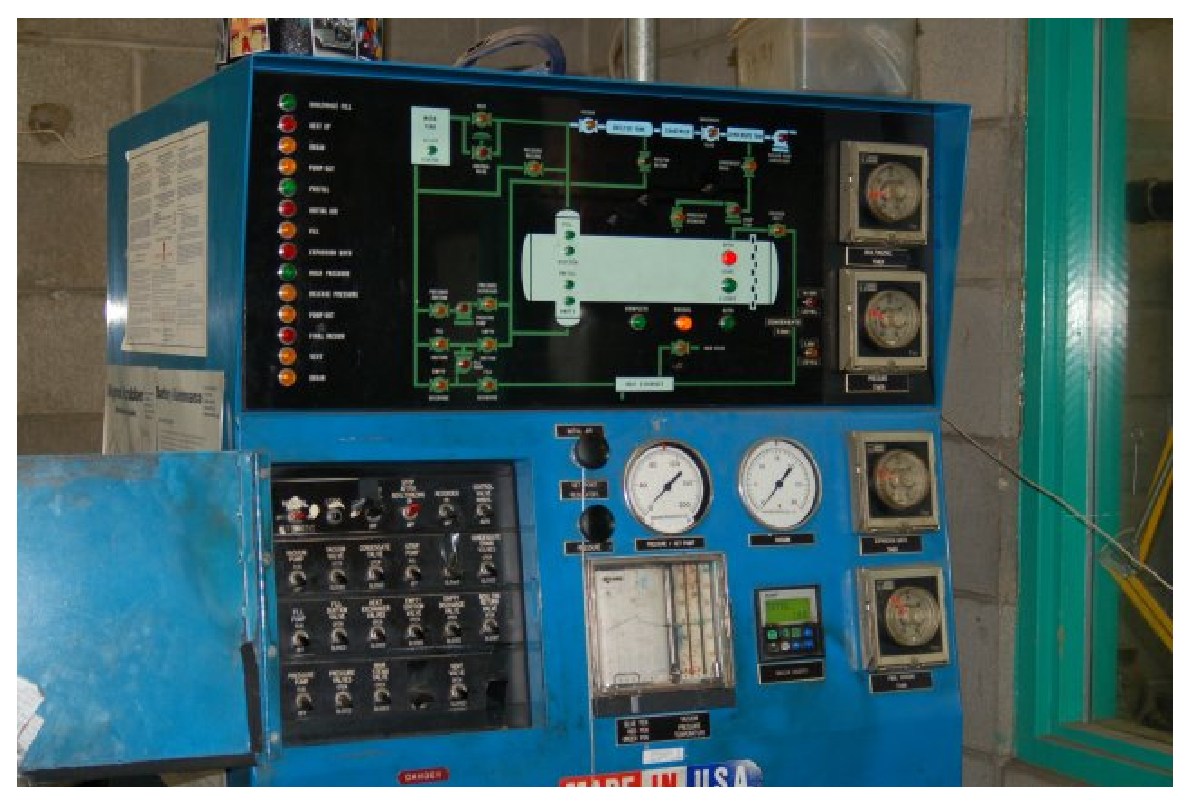
\includegraphics[width=3.5in]{i00001x13.eps}$$

\noindent
{\it En autoklav brukt til trykkimpregnering av trevirke.}






\vskip 10pt \filbreak

\noindent
{\bf Luft- og romfart:}

$$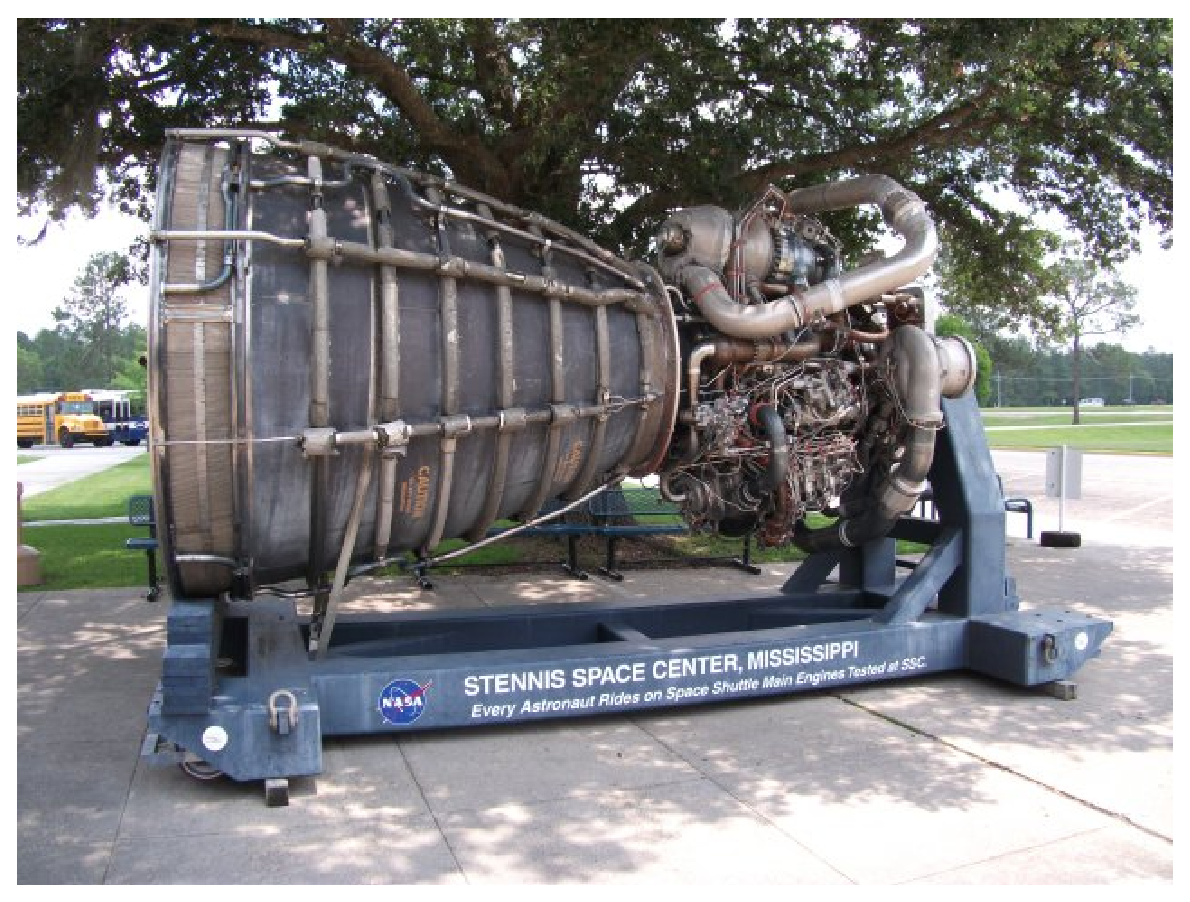
\includegraphics[width=5.5in]{i00001x14.eps}$$
$$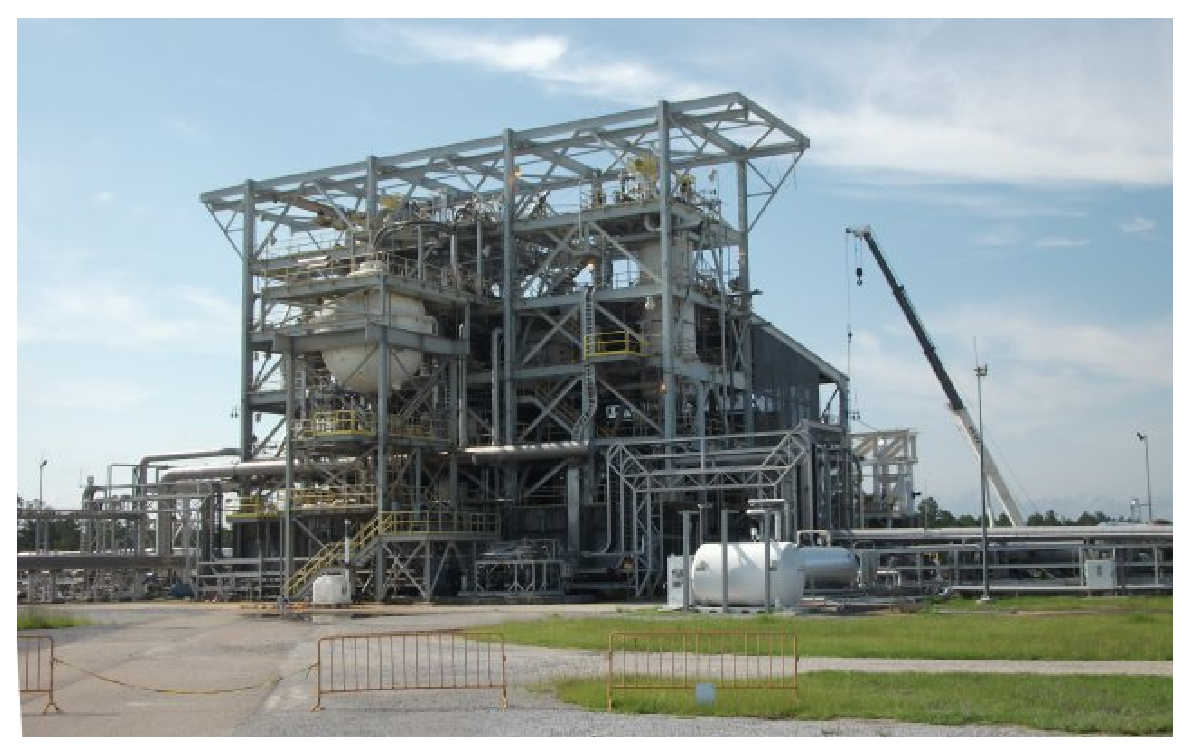
\includegraphics[width=5.5in]{i00001x18.eps}$$

\noindent
{\it Bilder tatt ved NASA sin rakettmotor-testfasilitet i Stennis, Mississippi.}






\vskip 10pt \filbreak

\noindent
{\bf Layout og design av instrumentstyringskretser:}

$$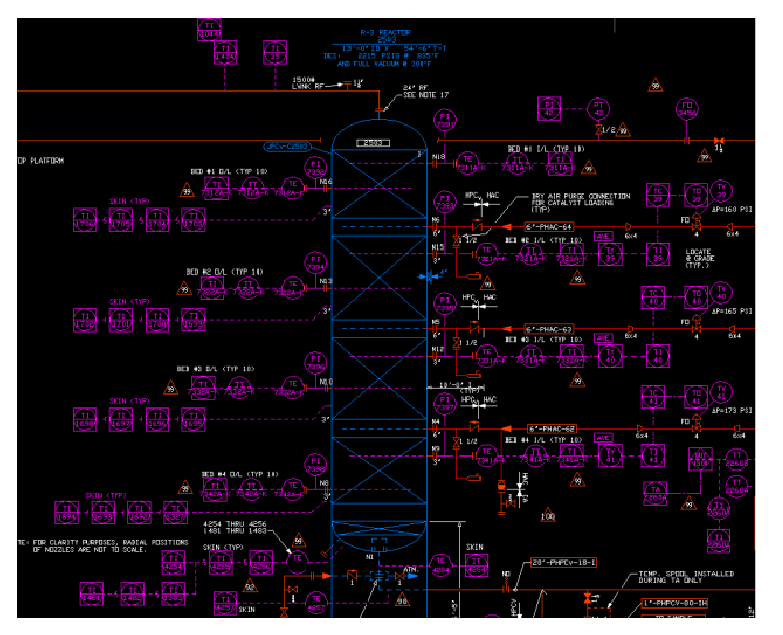
\includegraphics[width=5.5in]{i00001x15.eps}$$

\noindent
{\it Et typisk skjermbilde av AutoCAD brukt til å tegne en P\&ID for en oljeraffineri-enhet.}

$$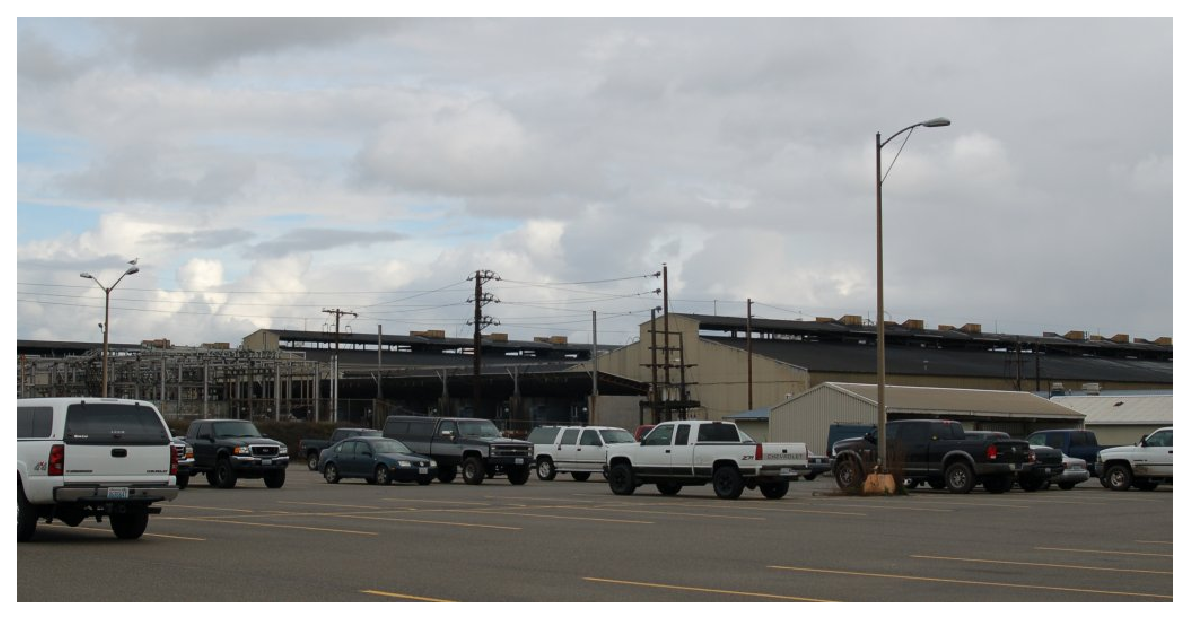
\includegraphics[width=5.5in]{i00001x38.eps}$$

\noindent
{\it ``Potline''-bygninger ved Alcoa/Intalco aluminiumsverk i Ferndale, Washington.}






\vskip 10pt \filbreak

\noindent
{\bf PLC-programmering (kontrollsystemdesign):}

$$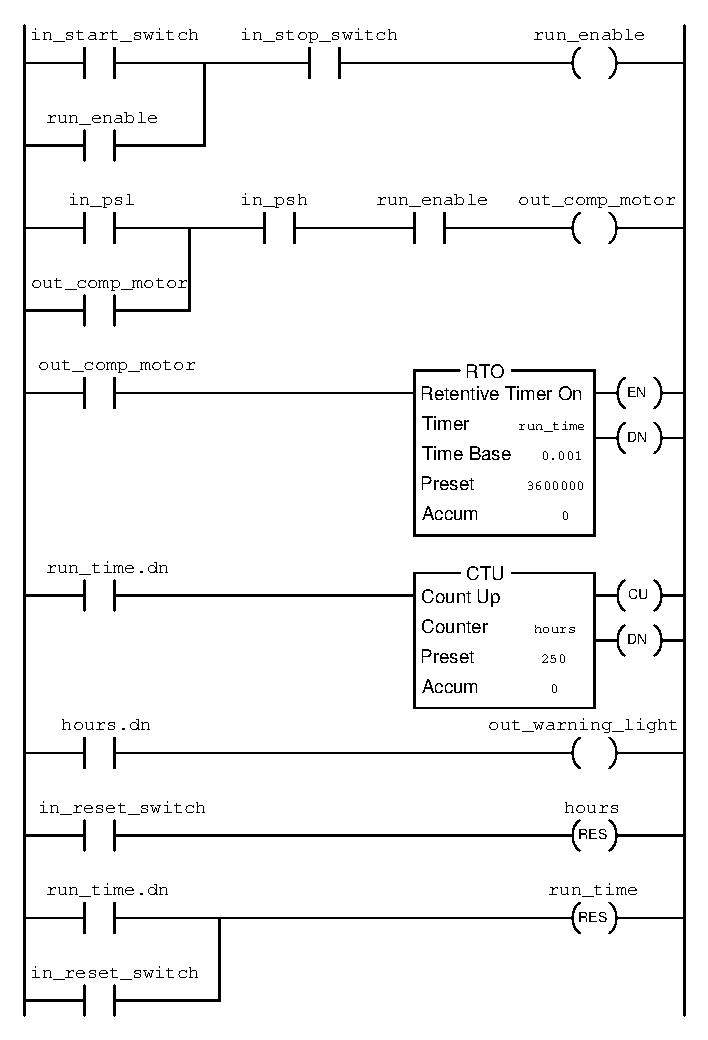
\includegraphics[width=15.5cm]{i00001x32.eps}$$

\noindent
{\it Et typisk PLC ``ladder logic''-program for en luftkompressor styrt av en Rockwell ControlLogix 5000 PLC er vist her.}






\vskip 10pt \filbreak

\noindent
{\bf Miljøovervåking:}

$$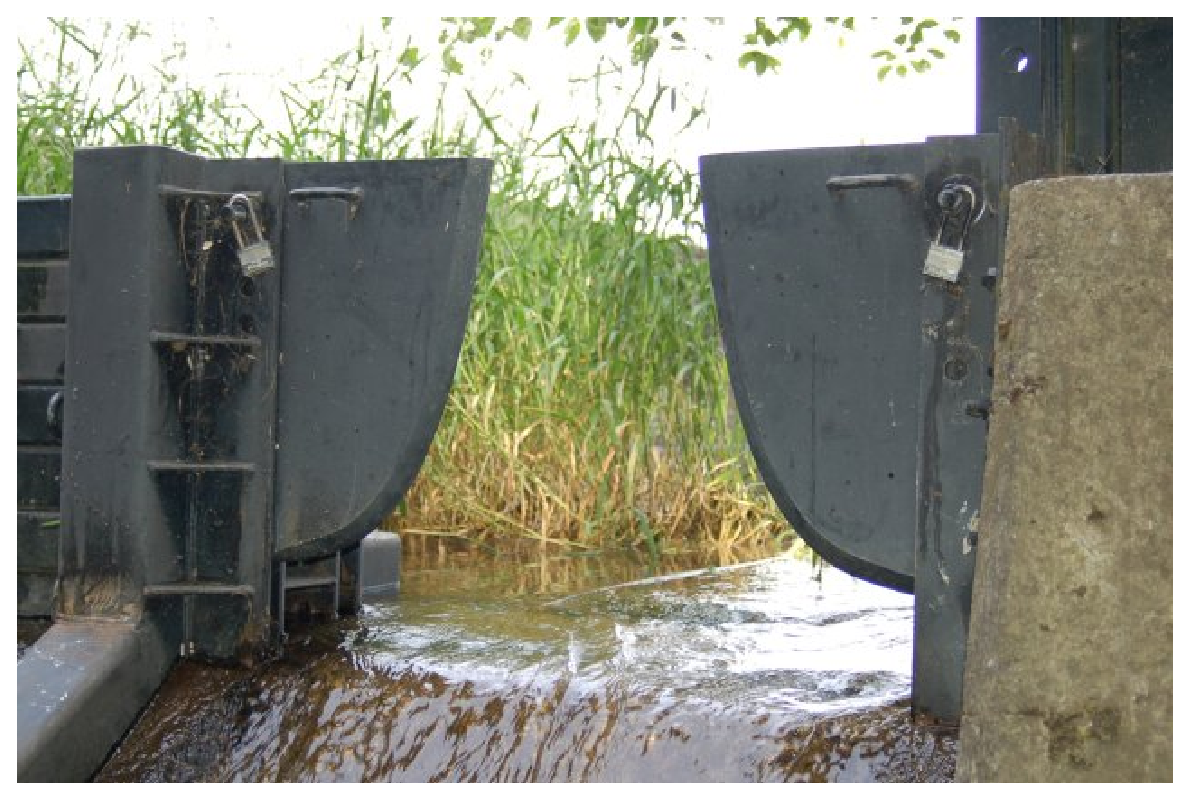
\includegraphics[width=4in]{i00001x17.eps}$$

\noindent
{\it Et Sutro-overfall brukt for å måle vannføringen ut av Lake Padden i Bellingham, Washington.}






\vskip 10pt \filbreak

\noindent
{\bf Energiforskning og -utvikling:}

$$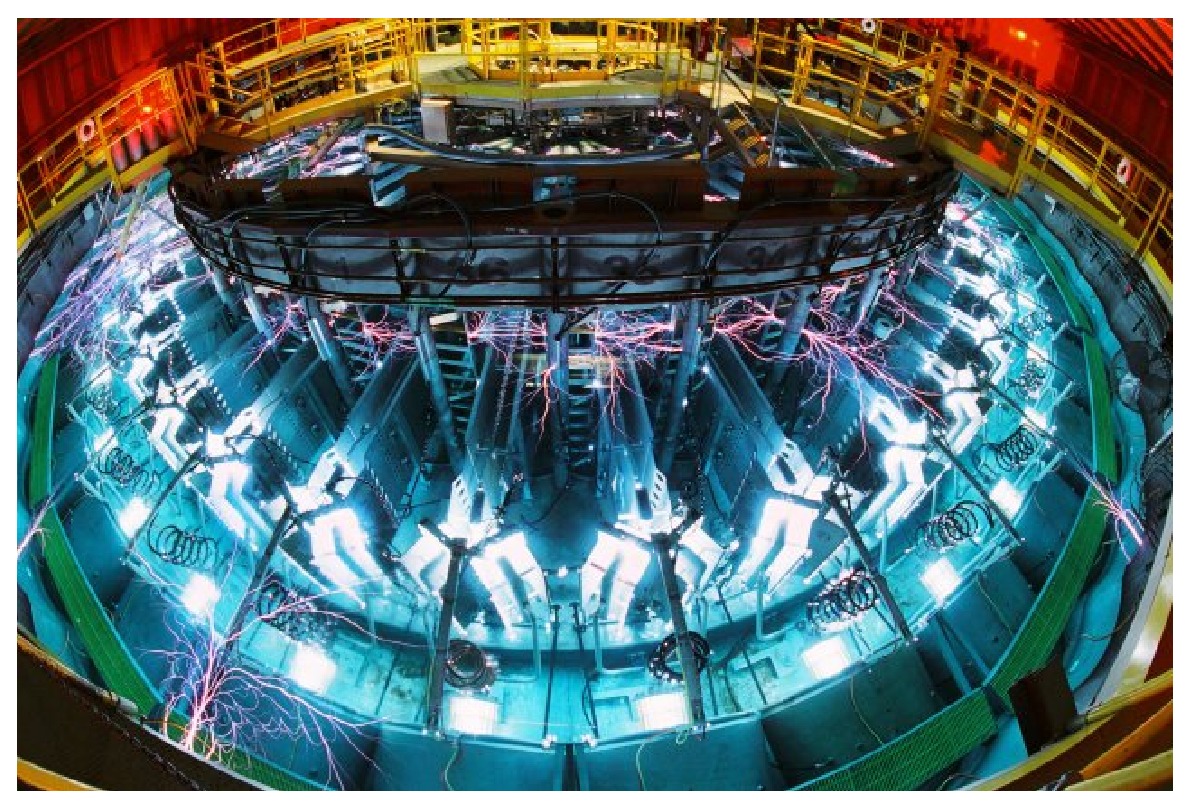
\includegraphics[width=3.5in]{i00001x22.eps}$$

\noindent
{\it Sandia National Laboratory sin pulserte kraftenhet brukt til eksperimenter innen kjernefusjon, og også til å teste effektene av elektromagnetisk pulsenergi på militært utstyr.  Foto: Department of Energy.}

\filbreak

$$
\includegraphics[width=3.5in]{i00001x41.eps}$$

{\it Kontrollrommet til Pacific Northwest National Laboratory sin Fast Flux Test-fasilitet, brukt til forskning på ``breeder''-reaktorteknologi for kjernefysjon.  Foto: Department of Energy.}





\vskip 10pt \filbreak

\noindent
{\bf Fornybar energi:}

$$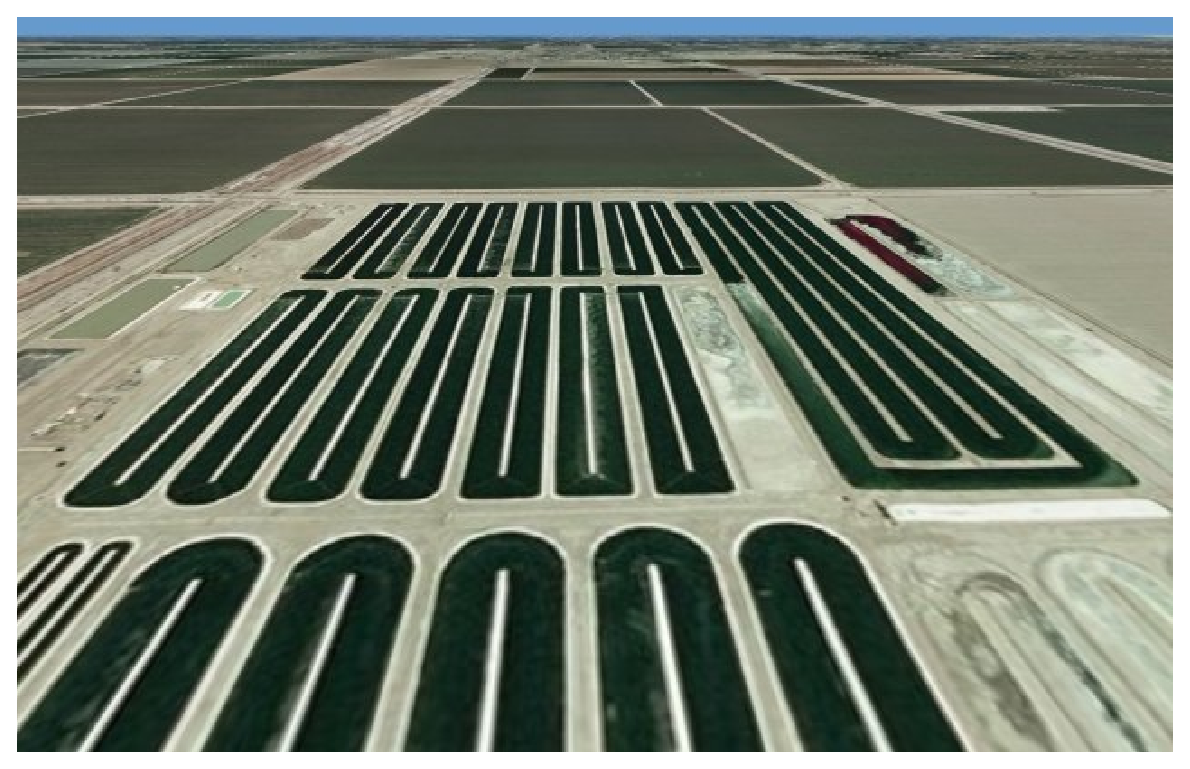
\includegraphics[width=3.5in]{i00001x21.eps}$$

\noindent
{\it Pacific Northwest National Laboratory sine eksperimentelle alge-dammer for sol-til-biomasse-konvertering.  Foto: Department of Energy.}

$$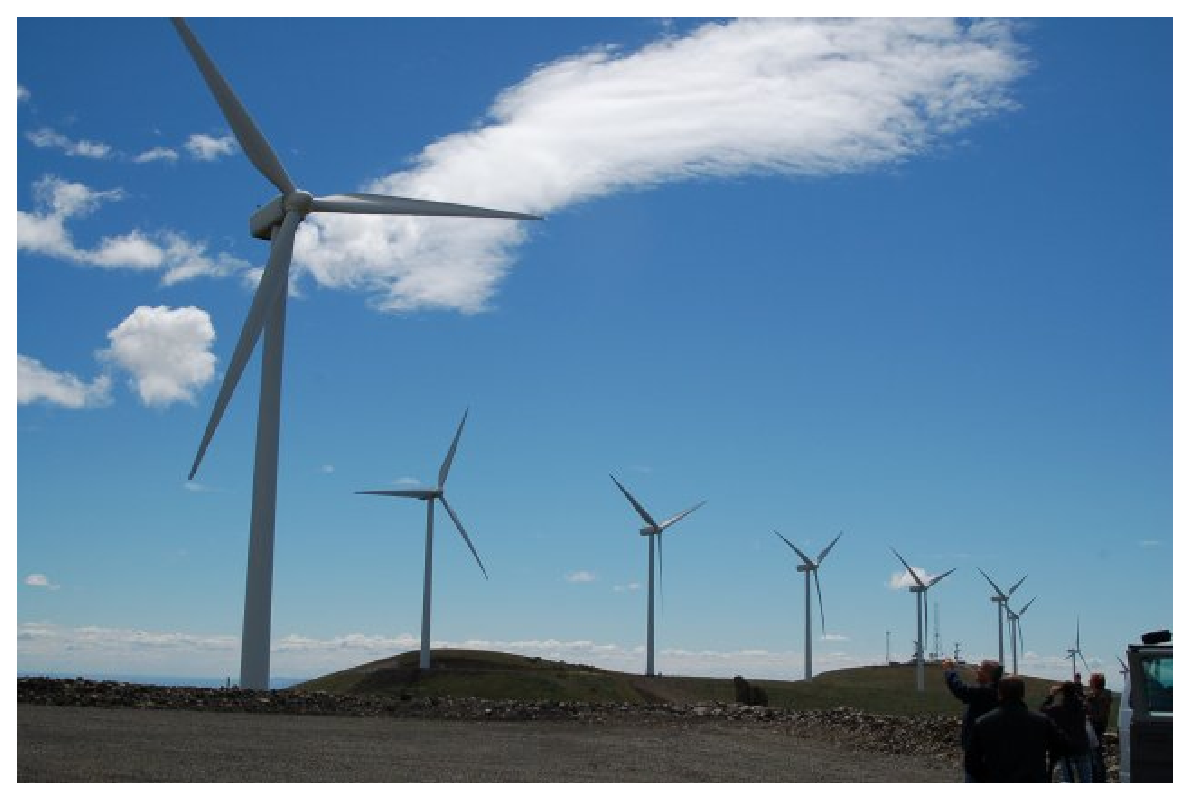
\includegraphics[width=3.5in]{i00001x24.eps}$$

\noindent
{\it Vindmøller ved Wild Horse vindpark nær Ellensburg, Washington, driftet av Puget Sound Energy.}

$$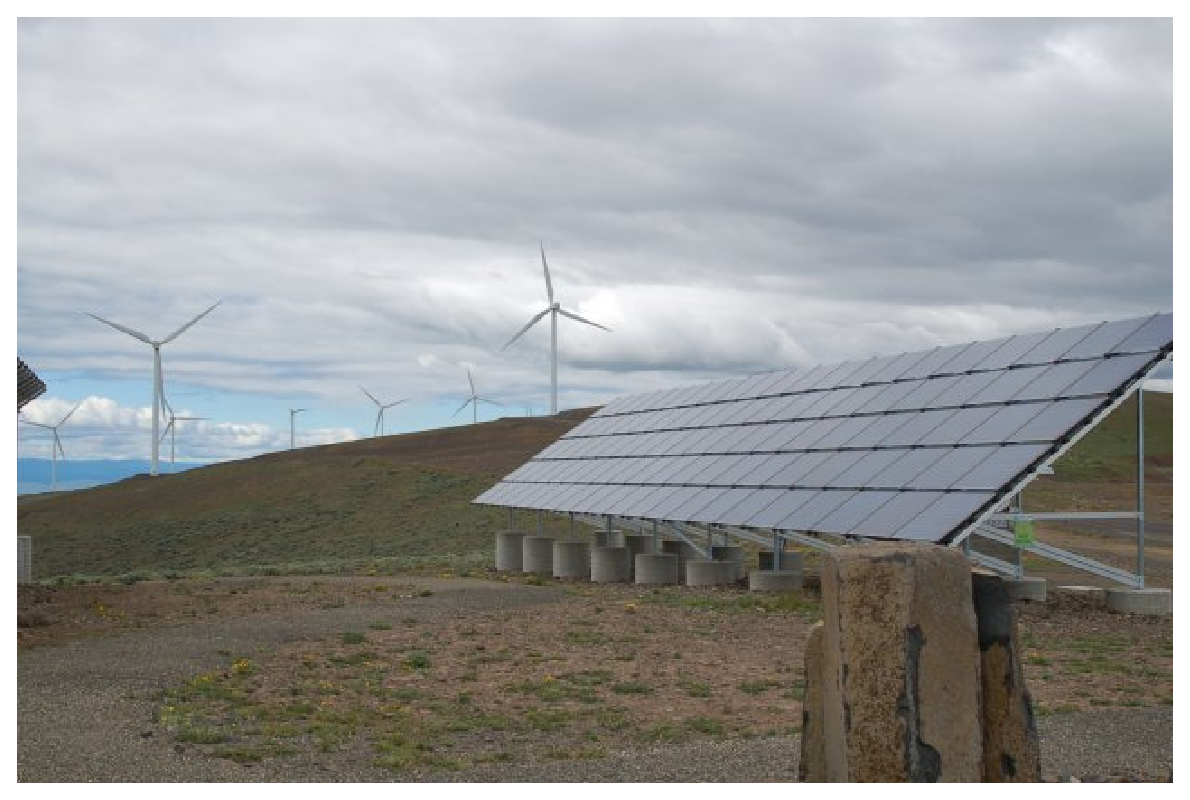
\includegraphics[width=3.5in]{i00001x25.eps}$$

\noindent
{\it Solcelleanlegg ved Wild Horse vindpark nær Ellensburg, Washington, driftet av Puget Sound Energy.}






\vskip 10pt \filbreak

\noindent
{\bf Gruvedrift:}

$$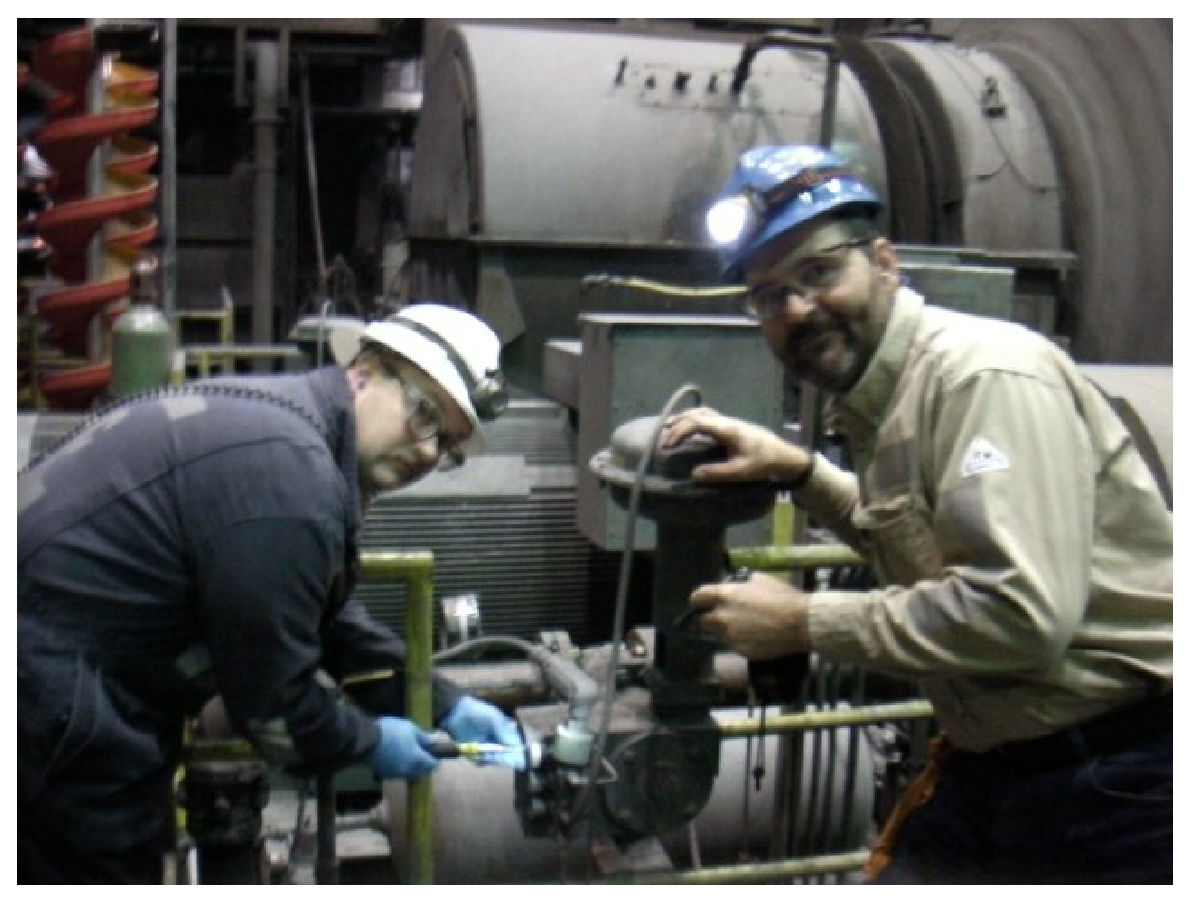
\includegraphics[width=4in]{i00001x20.eps}$$

\noindent
{\it BTC Instrumentation-graduates Micah og Mark som arbeider på en reguleringsventil nær en malmknuser i Alaska.}






\vskip 10pt \filbreak

\noindent
{\bf Service på reguleringsventiler:}

$$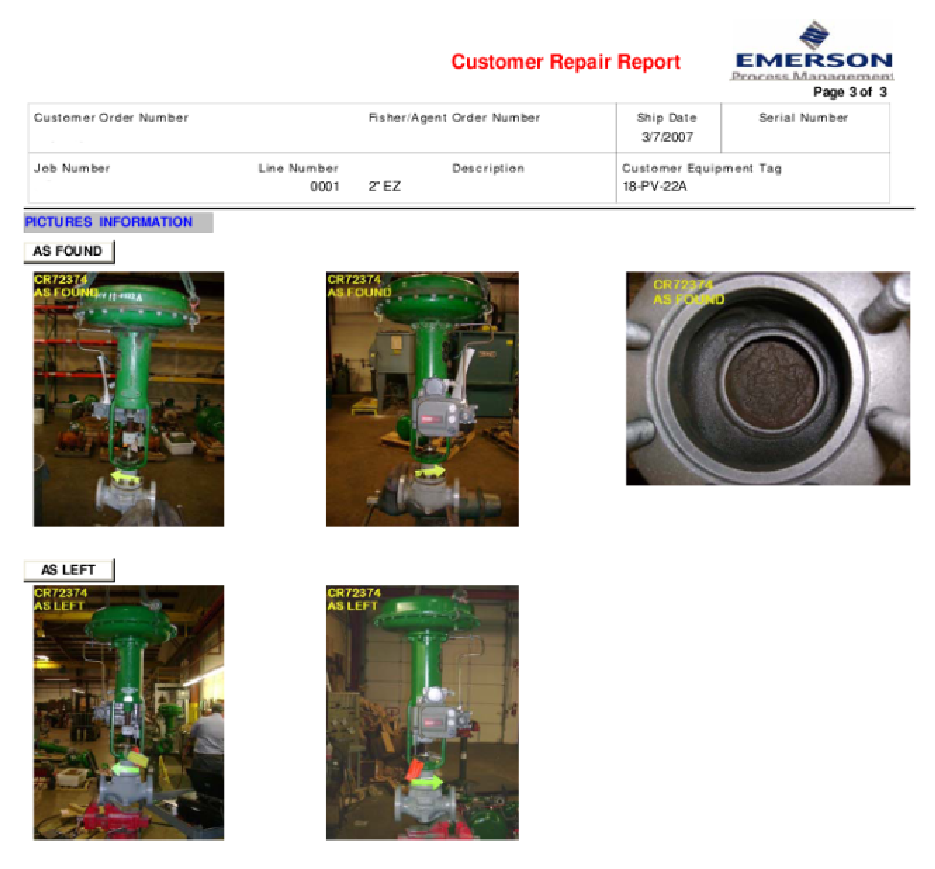
\includegraphics[width=15.5cm]{i00001x31.eps}$$

\noindent
{\it Typisk ``As-Found'' og ``As-Left''-side fra en rapport om overhaling av reguleringsventil.}






\vskip 10pt \filbreak

\noindent
{\bf Kontraktarbeid innen instrumentering:}

$$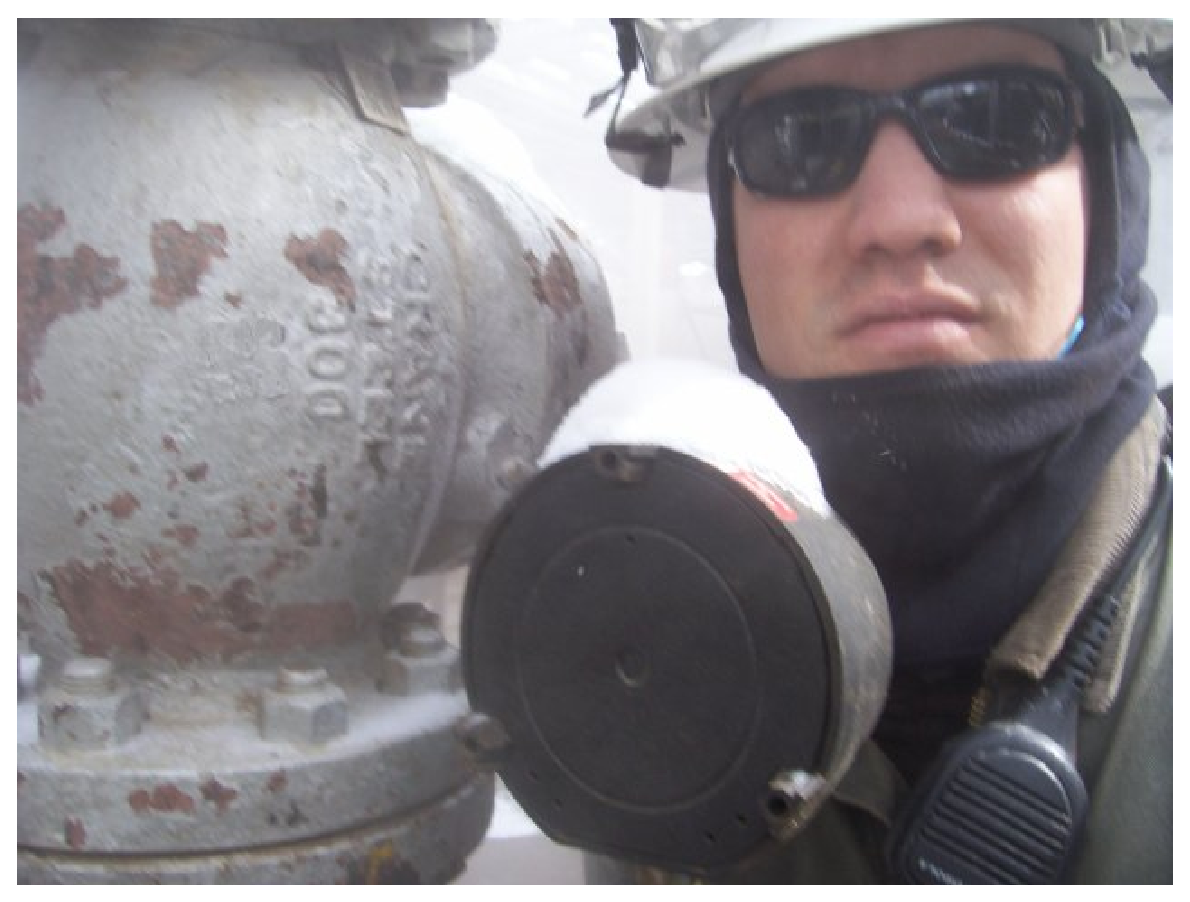
\includegraphics[width=4in]{i00001x23.eps}$$

\noindent
{\it BTC Instrumentation-graduate Corey utfører service på en reguleringsventil ved et oljeraffineri i Wyoming under en vinterstans.}

\vskip 10pt





Andre karrieresektorer som ikke er vist i denne bildesamlingen inkluderer (men er ikke begrenset til):

\begin{itemize}
\item{} Produksjonslinjer i industrien
\item{} Forskning og utvikling i bilindustrien
\item{} Service på vekter og veiematere
\item{} Kalibreringslaboratorier
\item{} Drift av universitetscampus sin infrastruktur
\item{} Geologisk overvåking (vulkanovervåking)
\item{} Robotikk
\item{} Vedlikehold av CNC-maskiner
\item{} Fjernstyrte kjøretøy
\item{} Salg av instrumentering
\end{itemize}

%(END_ANSWER)





%(BEGIN_NOTES)

Den samme undersøkelsen fra Washington State ga også en tankevekkende statistikk om opplæring på jobben.  Spørsmålet i undersøkelsen lød: ``Har bedriften din gitt minst 4 timer opplæring på jobb under en skriftlig plan til noen ansatte de siste 12 månedene?''  Svarene var bare 31\% ja og 69\% nei.

\vskip 10pt

Hvis du planlegger å gjennomgå de ulike bransjene som er avbildet i svarseksjonen (i fotografisk form), er et godt diskusjonsfokus å peke på noe av den videreopplæringen du sannsynligvis vil møte i hver bransje.  For eksempel:

\begin{itemize}
\item{} {\bf Elektrisk kraftproduksjon:} lære hvordan spesialiserte kontrollsystemer for elektriske generatorer fungerer, tilpasse seg endringer i bransjen som desentralisert kraftproduksjon (f.eks. vindparker, solgeneratorer, energilagringsanlegg).
\begin{itemize}

\item{} Eksempel: vernreléer
\item{} Eksempel: ``smart grid''-instrumentering
\item{} Eksempel: kryptering og sikkerhet i kontrollnettverk
\end{itemize}
\item{} {\bf Olje- og naturgassleting/produksjon:} lære å overvåke og regulere toppmoderne utvinningsteknologier som horisontal boring og dyphavsproduksjon, lære egenskapene til produksjonsprosesser for å optimalisere regulering og sikkerhetsnedstengning.
\begin{itemize}

\item{} Eksempel: horisontal boring
\item{} Eksempel: maksimere brønnytelse
\item{} Eksempel: custody transfer-instrumentering
\end{itemize}
\item{} {\bf Oljeraffinering:} få typer produksjonsanlegg tilbyr så mye teknologisk kompleksitet på ett sted som et oljeraffineri -- du kan bruke en hel karriere på å lære om prosessene og teknologiene som brukes i et typisk raffineri uten å nå slutten!
\begin{itemize}

\item{} Eksempel: katalytiske kjemiske reaksjonsprosesser
\item{} Eksempel: utvinning av farlige materialer (f.eks. vannfri ammoniakk, hydrogensulfid)
\item{} Eksempel: nye prosesser for raffinering av krevende råvarer som ``light tight oil'' fra Bakken-skiferen og andre felt
\end{itemize}
\item{} {\bf Kullgassifisering:} lære å måle og regulere relativt nye teknologier som slagging-gassifikatorer.
\begin{itemize}

\item{} Eksempel: utvinning av farlige materialer (f.eks. vannfri ammoniakk, hydrogensulfid)
\end{itemize}
\item{} {\bf Kjemisk prosessindustri:} disse anleggene er vanligvis svært varierte, og har en rekke høynivå-farer.
\begin{itemize}

\item{} Eksempel: utvinning av farlige materialer (f.eks. vannfri ammoniakk, hydrogensulfid)
\end{itemize}
\item{} {\bf Tremasse- og papirproduksjon:} en pulp- og papirmølle er nesten like mangfoldig som et oljeraffineri med hensyn til instrumentering.  En ekstra teknisk utfordring med eldre papirmøller er at de ofte bruker alt fra gamle pneumatiske instrumenter til de nyeste toppmoderne systemene -- med andre ord blir gammel teknologi ikke oppdatert like ofte som i et oljeraffineri.
\begin{itemize}

\item{} Eksempel: ``hog fuel''-kjelekontroller, utfordrende på grunn av den inkonsistente naturen til treavfall (``hog'')-brensel
\item{} Eksempel: recovery boiler-operasjoner (svært farlige prosesser, kjent for sin historikk med eksplosive feil)
\end{itemize}
\item{} {\bf Farmasøytisk produksjon:} lære produksjonskravene for nye produktlinjer, lære å kalibrere og vedlikeholde det nyeste innen biologisk instrumentering.
\item{} {\bf Næringsmiddelindustri og emballering:} lære å bruke automasjon for å redusere kostnader og øke tilgjengeligheten av mat.
\item{} {\bf Alkoholproduksjon og tapping:} lære å bruke automasjon i småskala håndverksbryggeri/destilleri-operasjoner.
\item{} {\bf Kommunal vann- og avløpsrensing:} lære å vedlikeholde de spesialiserte instrumentene som brukes til å måle vannkvalitet, og hvordan man kontrollerer nye prosesser for å rense vannet.
\begin{itemize}

\item{} Eksempel: nye prosesser for behandling av vann forurenset med medisinsk avfall
\end{itemize}
\item{} {\bf Elektrisk kraftproduksjon:} lære hvordan spesialiserte kontrollsystemer for elektriske generatorer fungerer, tilpasse seg endringer i bransjen som desentralisert kraftproduksjon (f.eks. vindparker, solgeneratorer, energilagringsanlegg).
\begin{itemize}

\item{} Eksempel: ``smart grid''-instrumentering
\item{} Eksempel: kryptering og sikkerhet i kontrollnettverk
\end{itemize}
\item{} {\bf Layout og design av instrumentstyringskretser:} lære nye programvarepakker som {\tt InTools} for dokumentasjon av instrumenteringssystemer.
\item{} {\bf PLC-programmering (kontrollsystemdesign):} lære nye merker og modeller av PLC-er, samt nye programmeringsspråk.
\item{} {\bf Fornybar energi:} alle utfordringene ved et vanlig kraftproduksjonsanlegg, pluss kompleksiteten til en energikilde som varierer ukontrollerbart!
\item{} {\bf Gruvedrift:} lære om den spesialiserte instrumenteringen brukt til å analysere malm i sanntid, pluss utfordringene ved å kontrollere maskineri og prosesser i ekstremt tøffe forhold.
\item{} {\bf Service på reguleringsventiler:} lære å bruke toppmoderne ``smart'' instrumentering til styring av store ventilmekanismer, lære om metallurgi og prosessvæskereaksjoner for å diagnostisere tidlige ventilfeil.
\item{} {\bf Kontraktarbeid innen instrumentering:} hver dag bringer en ny utfordring ettersom arbeidet stadig endrer karakter og sted!
\end{itemize}



I interessen av å ha nok tid til å gjennomføre mastery-eksamenen, bør gjennomgangen av disse ulike bransjene være kort.

%INDEX% Career, range of industries

%(END_NOTES)
